\documentclass[11pt]{article}
\usepackage{amsmath}
\usepackage{graphicx}
\usepackage{color}
\usepackage{longtable}
\usepackage{tabu} %% text tables
%%\usepackage[linktocpage=true]{hyperref} %% links to numbers instead of sections
\usepackage{hyperref}
%%\usepackage{url}
\usepackage{geometry}
\geometry{left=3.5cm,right=3.5cm,top=3.5cm,bottom=3.5cm}
\graphicspath{{./WP_images/}}
%%\usepackage{cite} 
%%\usepackage{notoccite}
\usepackage[backend=bibtex,sorting=none]{biblatex}
\addbibresource{wp-refs.bib}




\begin{document}
\title{%
Basic Attention Token (BAT) White Paper\\
\large Blockchain Based Digital Advertising}
\author{Brave Software}
\date{March 21, 2017}

\maketitle

%\setcounter{tocdepth}{2}
\tableofcontents


%% \section{Overview}
%% \label{sec-1}
\begin{abstract}
%% \item{Digital advertising is broken. }
%% \item{The marketplace for online advertising, once dominated by advertisers, publishers and users, has become overrun by “middleman” ad exchanges, audience segmentation, complicated behavioral and cross-device user tracking, and opaque cross-party sharing through data management platforms.}
%% \item{Publishers lose billions of dollars to increasing levels of fraud and faulty means of accurately attributing user attention. }
%% \item{Users face unprecedented levels of malvertisements and privacy violations. Mobile advertising results on average \$23 per month in data charges, slow page loads, and 21\% less battery life.  }
%% \item{In response, over 600 million mobile devices and desktops (globally) employ ad blocking software and this number is growing quickly. }
%% \item{This crisis for traditional publishers is now exacerbated by the rise of Google and Facebook, which together claim 73\% of digital ad revenue and 99\% of all growth. }
%% \item{Traditional publishers have lost approximately 66\% of their revenue over the last 12 years, adjusted for inflation. }
%% \item{Publishers face falling revenue, users feel increasingly violated, and advertisers’ ability to assess effectiveness is diminished. }
%% \item{The solution is a decentralized, transparent digital ad exchange based on Blockchain. }
%% \item{The first component is Brave, a fast, open source, privacy-focused browser that blocks third party ads and trackers, and builds in a ledger system that captures user attention to  reward publishers accordingly. }
%% \item{Brave will now introduce BAT (Basic Attention Token), a token for a decentralized ad exchange. It compensates the browser user for attention while guaranteeing privacy.}
%% \item{BAT connects advertisers, publishers, and users and is denominated by relevant user attention, while removing social and economic costs associated with existing ad networks, e.g., fraud, privacy violations, and malvertising.}
%% \item{BAT is a payment system that rewards and protects the user while giving better conversion to advertisers and higher yield to publishers.}
%% \item{We see BAT and associated technologies as a future part of web standards, solving the important problem of monetizing publisher content while protecting user privacy. }
Digital advertising is broken. 
The marketplace for online advertising, once dominated by advertisers, publishers and users, has become overrun by “middleman” ad exchanges, audience segmentation, complicated behavioral and cross-device user tracking, and opaque cross-party sharing through data management platforms.
Publishers lose billions of dollars to increasing levels of fraud and faulty means of accurately attributing user attention. 
Users face unprecedented levels of malvertisements and privacy violations. Mobile advertising results on average \$23 per month in data charges, slow page loads, and 21\% less battery life.  
In response, over 600 million mobile devices and desktops (globally) employ ad blocking software and this number is growing quickly. 
This crisis for traditional publishers is now exacerbated by the rise of Google and Facebook, which together claim 73\% of digital ad revenue and 99\% of all growth. 
Traditional publishers have lost approximately 66\% of their revenue over the last 12 years, adjusted for inflation. 
Publishers face falling revenue, users feel increasingly violated, and advertisers’ ability to assess effectiveness is diminished. 
The solution is a decentralized, transparent digital ad exchange based on Blockchain. 
The first component is Brave, a fast, open source, privacy-focused browser that blocks third party ads and trackers, and builds in a ledger system that captures user attention to  reward publishers accordingly. 
Brave will now introduce BAT (Basic Attention Token), a token for a decentralized ad exchange. It compensates the browser user for attention while guaranteeing privacy.
BAT connects advertisers, publishers, and users and is denominated by relevant user attention, while removing social and economic costs associated with existing ad networks, e.g., fraud, privacy violations, and malvertising.
BAT is a payment system that rewards and protects the user while giving better conversion to advertisers and higher yield to publishers.
We see BAT and associated technologies as a future part of web standards, solving the important problem of monetizing publisher content while protecting user privacy. 

\end{abstract}

\section{Value Proposition}
\label{sec-2}

We propose the BAT as a token of exchange in a secure, anonymous, opt-in advertising system based in the browser and the mobile app webview. The BAT system provides: 
\begin{itemize}
\item{Users: strong privacy and security when viewing advertisements, improved relevance and performance, and a share of tokens. }
\item{Publishers: improved  revenue, better reporting, and less fraud. }
\item{Advertisers: less expensive customer attention, less fraud, and better attribution.}
\end{itemize}
\section{Introduction}
\label{sec-3}

\begin{quote}\textit{“Attention has been widely recognized as a commodity, like wheat, pork bellies or crude oil. Existing industries have long depended on it to drive sales. And the new industries of the twentieth century turned it into a form of currency they could mint. Beginning with radio, each new medium would attain its commercial viability through the resale of what attention it could capture in exchange for its ‘free’ content.”} -Tim Wu, Attention Brokers \end{quote} 

The promise of advertising technology (“ad-tech”) was to create a more efficient marketplace for attention. The hope was that the Internet, the latest kind of “new medium,” would arrive with a transparent and efficient ad marketplace. 

In theory, excellence would be rewarded. The best journalism and entertainment would receive the attention and funding it deserved. Ad tech would “get marketers closer to their users via data analysis, immediate valuation and distribution.” Data would be used to “accurately identify audiences, determine the value of those audiences, and deliver the right messages to them instantly.”\cite{1} In short, users’ attention would be valued properly. 

That didn’t happen. Instead, the ad-tech ecosystem that has evolved over the last two decades is a bewildering variety of middlemen and complexity. Worse, ad-tech introduced a host of correlated problems for publishers, advertisers and users. Users have lost their privacy, face increasing malware, pay high charges to download ads, and suffer slow speeds. Publishers have lost billions in revenue while fraud has skyrocketed. And advertisers face poor reporting and targeting.  

This paper will review the current state of ad-tech and the predicament of content producers. It will outline a new solution that creates a transparent and efficient Blockchain-based marketplace for publishers, advertisers and users, accurately valuing and rewarding the key driver of Internet content: durable user attention. 
\subsection{An Inefficient and Troubled Market}
\label{sec-3-1}

Thomas Davenport and JC Beck note that “attention is focused mental engagement on a particular item of information. Items come into our awareness, we attend to a particular item, and then we decide whether to act.”\cite{2} Attention is, in this sense, a form of scarcity, which raises fundamental economic questions, which we shall address momentarily.
 
Advertising, throughout history, has been used as the primary mechanism to capture Attention, raise it to a level of Interest to incite some Desire that can then translate it into Action -- otherwise known as AIDA.\cite{3} The earliest forms of advertising date to ancient China, Egypt and the Middle Ages in Europe. The print form of advertising began to expand widely with the growth of 19th Century printed products. This marketplace of advertisers, publishers and users remained relatively straightforward -- despite some additions -- even as the new media of radio and television arose. 

The rise of the Internet brought the development of a new level of advertising technology with the promise of higher speed and better information, two critical elements that had the potential to radically improve the efficiency of the attention marketplace. Somewhat counter-intuitively, the sheer complexity and opacity that organically developed has brought the opposite result. The system isn’t working as it should. As the Chief Brand officer of the largest advertiser, P\&G, said recently: \begin{quote}\textit{``The days of giving digital a pass are over. It's time to grow up. It's time for action.''}\cite{4}\end{quote}

Especially in the last decade, the advertising ecosystem has become more complex and crowded, with many more players taking a piece of the advertising pie, either directly or indirectly. The complexity of this ecosystem increases the cost in headcount and difficulty of the tasks for the digital marketing teams on the advertiser's side. At the other end of the system, the typical publisher faces both a shrinking market for the ad-blocker-free attention, and a shrinking slice of the advertising revenue pie due to the multitude of third party players who act as economic middlemen in the transaction. 

\subsection{The Attention Marketplace:}
\label{sec-3-2}

Sales planners currently budgeting for brand advertising are required to account for an excessive number of intermediaries that stand between the ad and the end user. Agencies, trading desks, demand side platforms, desktop and mobile network exchanges, yield optimization, rich media vendors and partnered services often consume significant portions of creative and delivery ad budget. It is also common for agencies in charge of packaging brand campaigns to use data aggregators, data management platforms, data suppliers, analytics, measurement and verification services to fight fraud, enhance targeting, and confirm attribution. All of these factors add up to a high transaction cost on the efficient provision of attention to brand ad campaigns.

\begin{center}
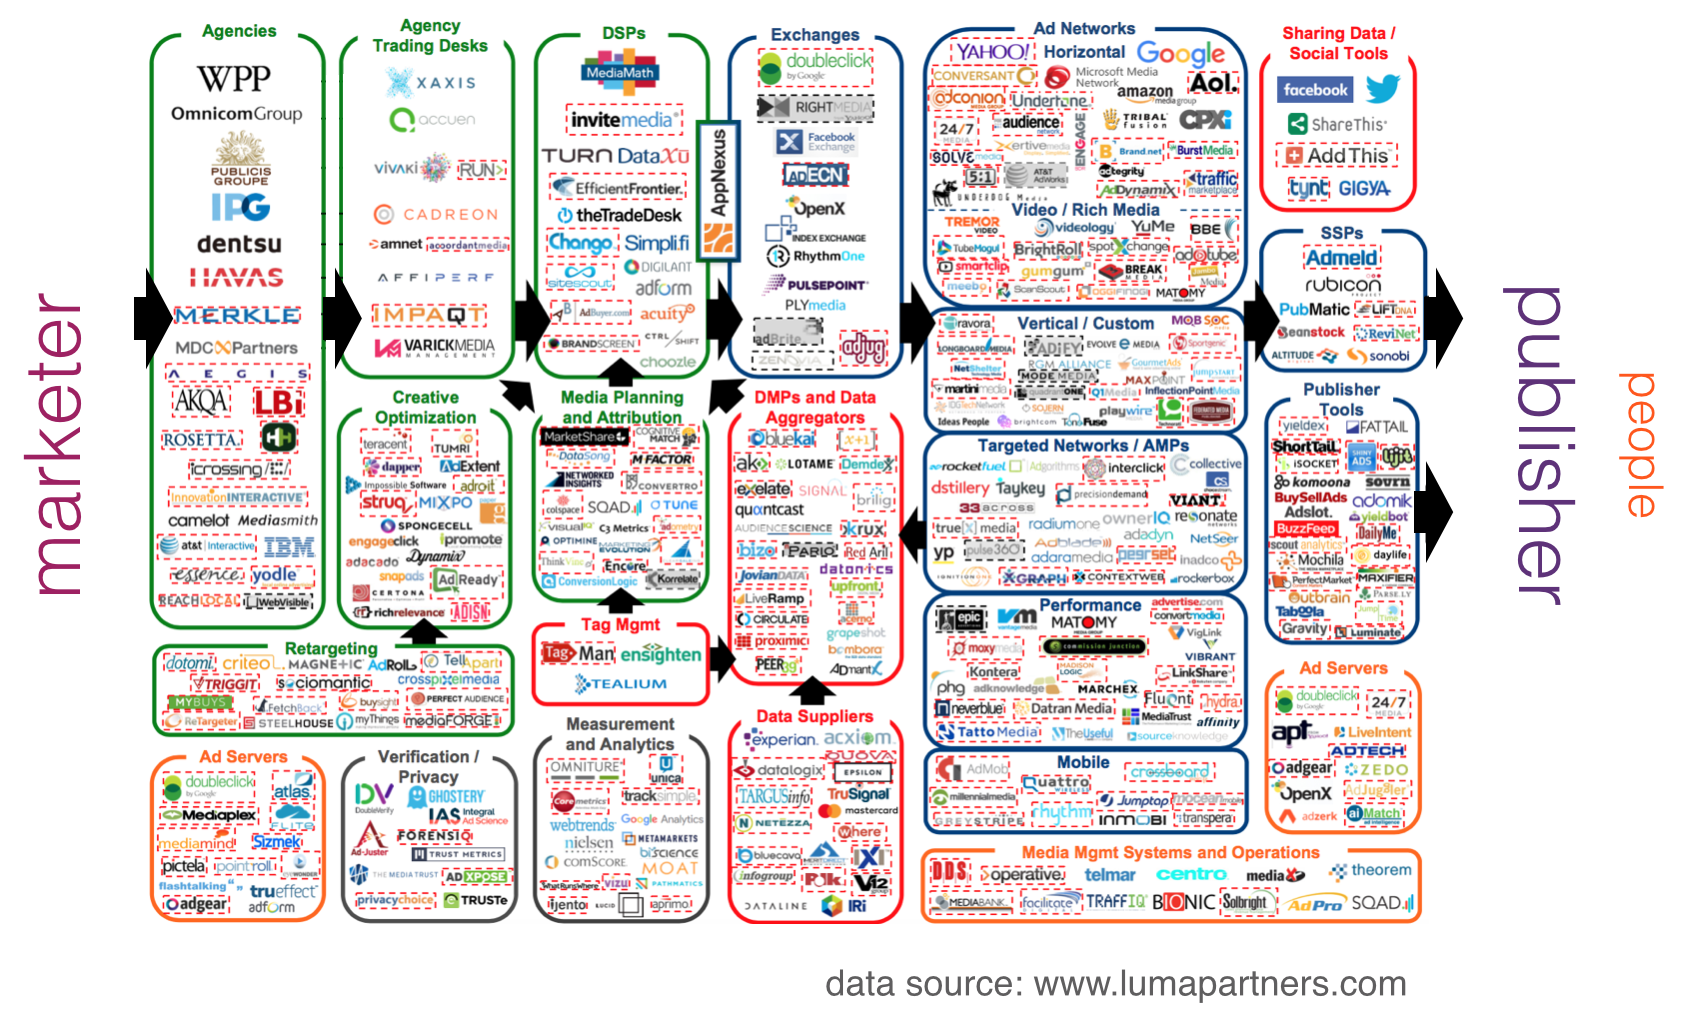
\includegraphics[width=0.9\textwidth]{lumascape_recolored.png}
\end{center}

Publishers also face a number of costs and intermediaries on the receiving side of the ads served. Publishers pay ad serving fees, operational fees for campaign setup, deployment and monitoring, publisher analytics tools; also they give up substantial revenue to some of the same intermediaries that the brand advertisers use via programmatic ads. Publishers face direct costs of user complaints when malvertising spreads from exchanges to loyal readers, often with little or no idea of origin and with no help from the ad exchanges responsible for allowing such ads to serve from their systems. All of these diminish net revenue, and the overall complexity of the advertising ecosystem raises headcount and expense.

\begin{figure}
\begin{center}
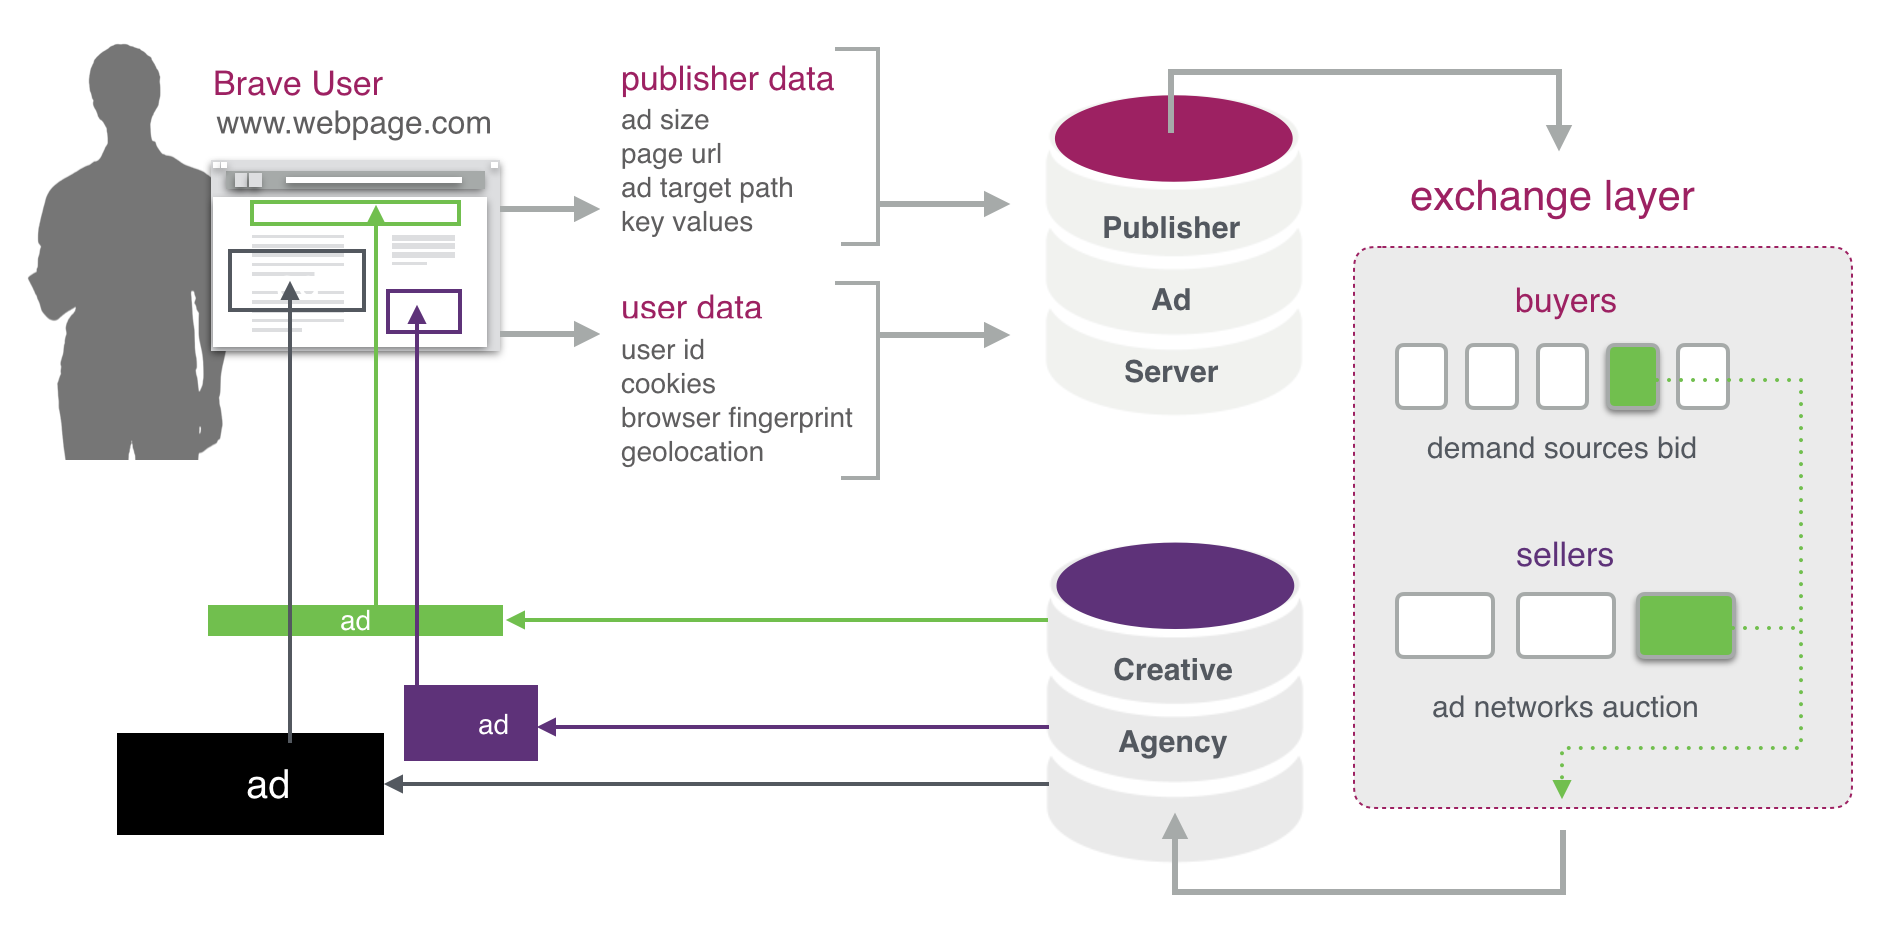
\includegraphics[width=0.9\textwidth]{typical_display_adflow.png}
\caption{Typical Digital Ad Flow}
\end{center}
\end{figure}

There is a hidden cost to this complexity. A single ad unit may bounce across many networks, buy and sell-side ad servers, verification partners and data management platforms. Publishers lose revenue from each middleman transaction. Each one of these transactions also detracts from the user experience. Many of the middle players involve data transfers, which add latency. Any transfers done via script on page eat into the user's data plan and battery life on mobile. Users often find their experience further diminished when the results finally arrive, confounded by a bewildering array of distracting ads the publisher allowed to be placed in hope of greater revenue. 

\begin{figure}
\begin{center}
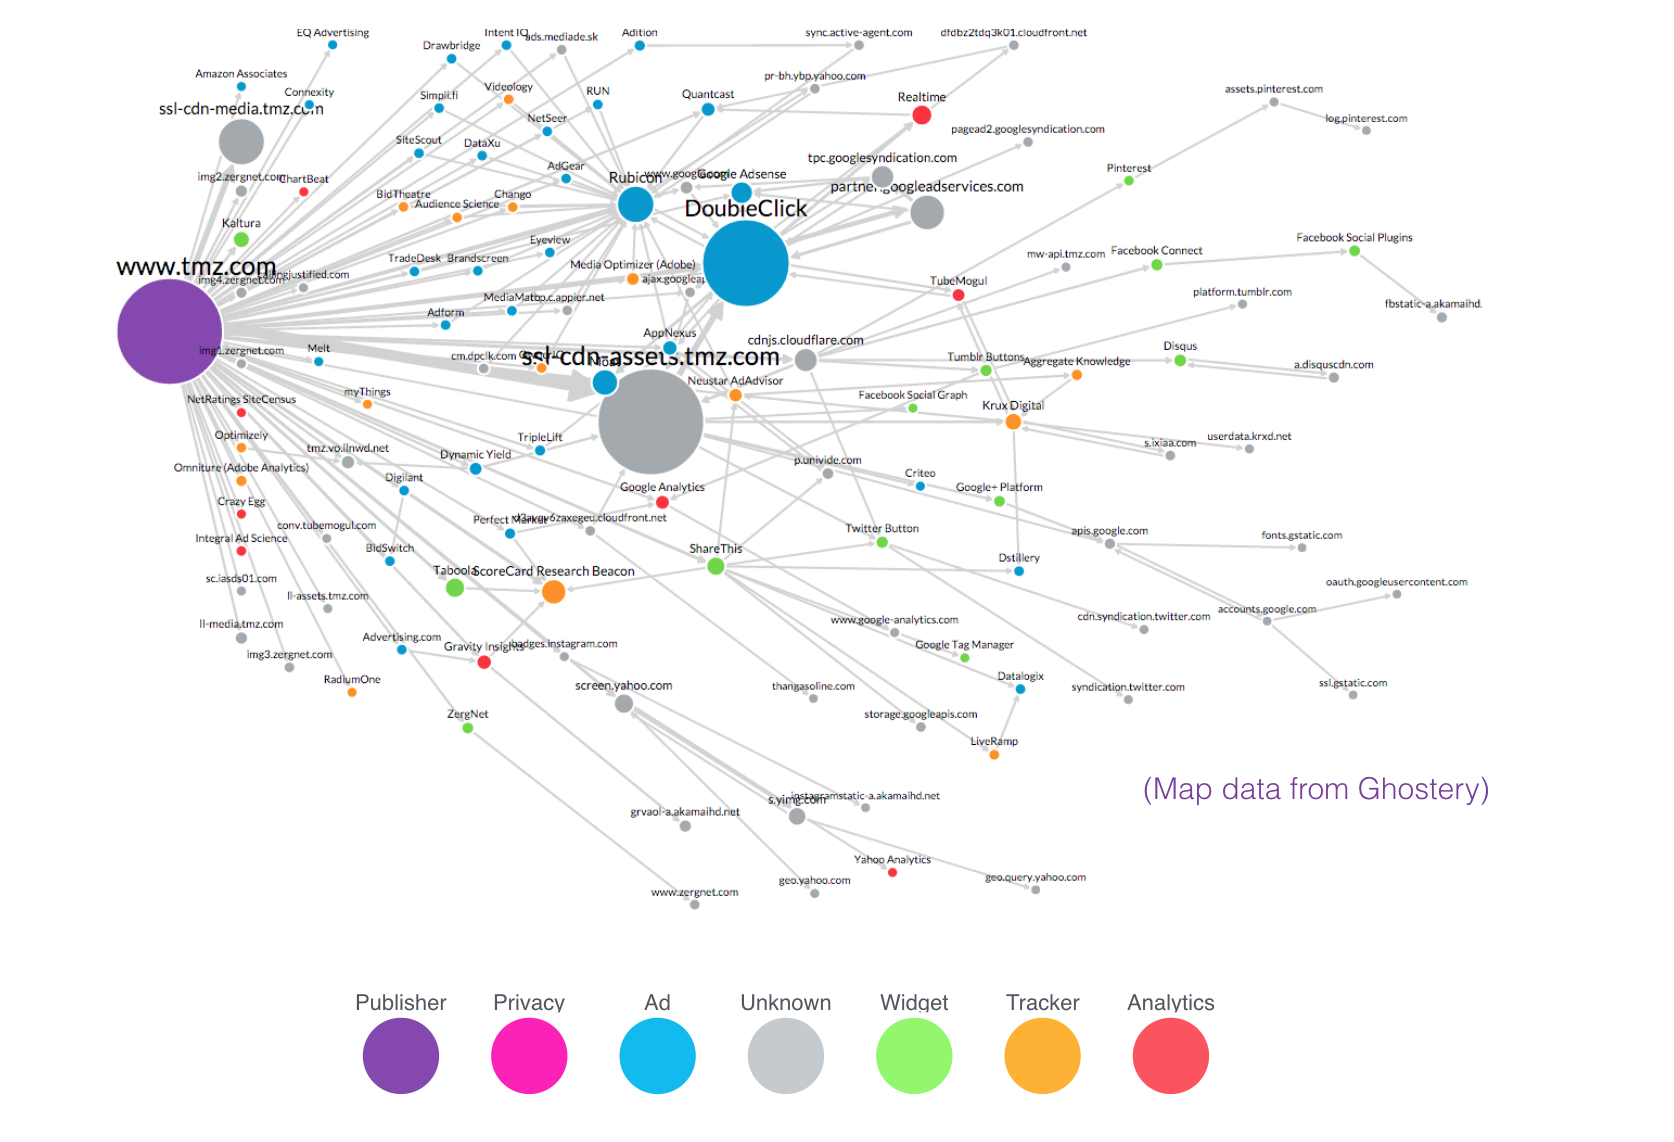
\includegraphics[width=0.9\textwidth]{tracking_map.png}
\caption{Typical Tracking on Large Content Sites}
\end{center}
\end{figure}

In addition, the violation of user privacy exacts a significant social cost; economists have compared violations of user privacy as analogous to environmental pollution.\cite{5} According to Pew Research, “Fully 91\% of adults agree or strongly agree that users have lost control of how personal information is collected and used by companies.”\cite{6} A large majority, 64\%, believe that the “government should do more to regulate advertisers” regarding how they use and store personal information. This is not surprising, given that a visit to a popular media site can often have 70 trackers set loose on the reader. 

Fraud is also a major problem afflicting the advertising marketplace. Hackers  create malicious bots that produce bogus websites that fool advertisers. Internet “bots” — remote-controlled software running on compromised personal computers or cloud infrastructure programmed to engage in criminal activities — siphon billions of dollars each year from the ad industry. According to Business Intelligence: “These bots create websites filled with infringed content and generate fake traffic through a complex network of infected computers. In 2016, ad fraud created by internet bots is expected to cost advertisers \$7.2 billion, up from \$6.3 billion in 2015, according to a report from the Association of National Advertises (ANA) and White Ops.”\cite{7} There is no sign of this level of fraud leveling off or reducing. 

\begin{figure}
\begin{center}
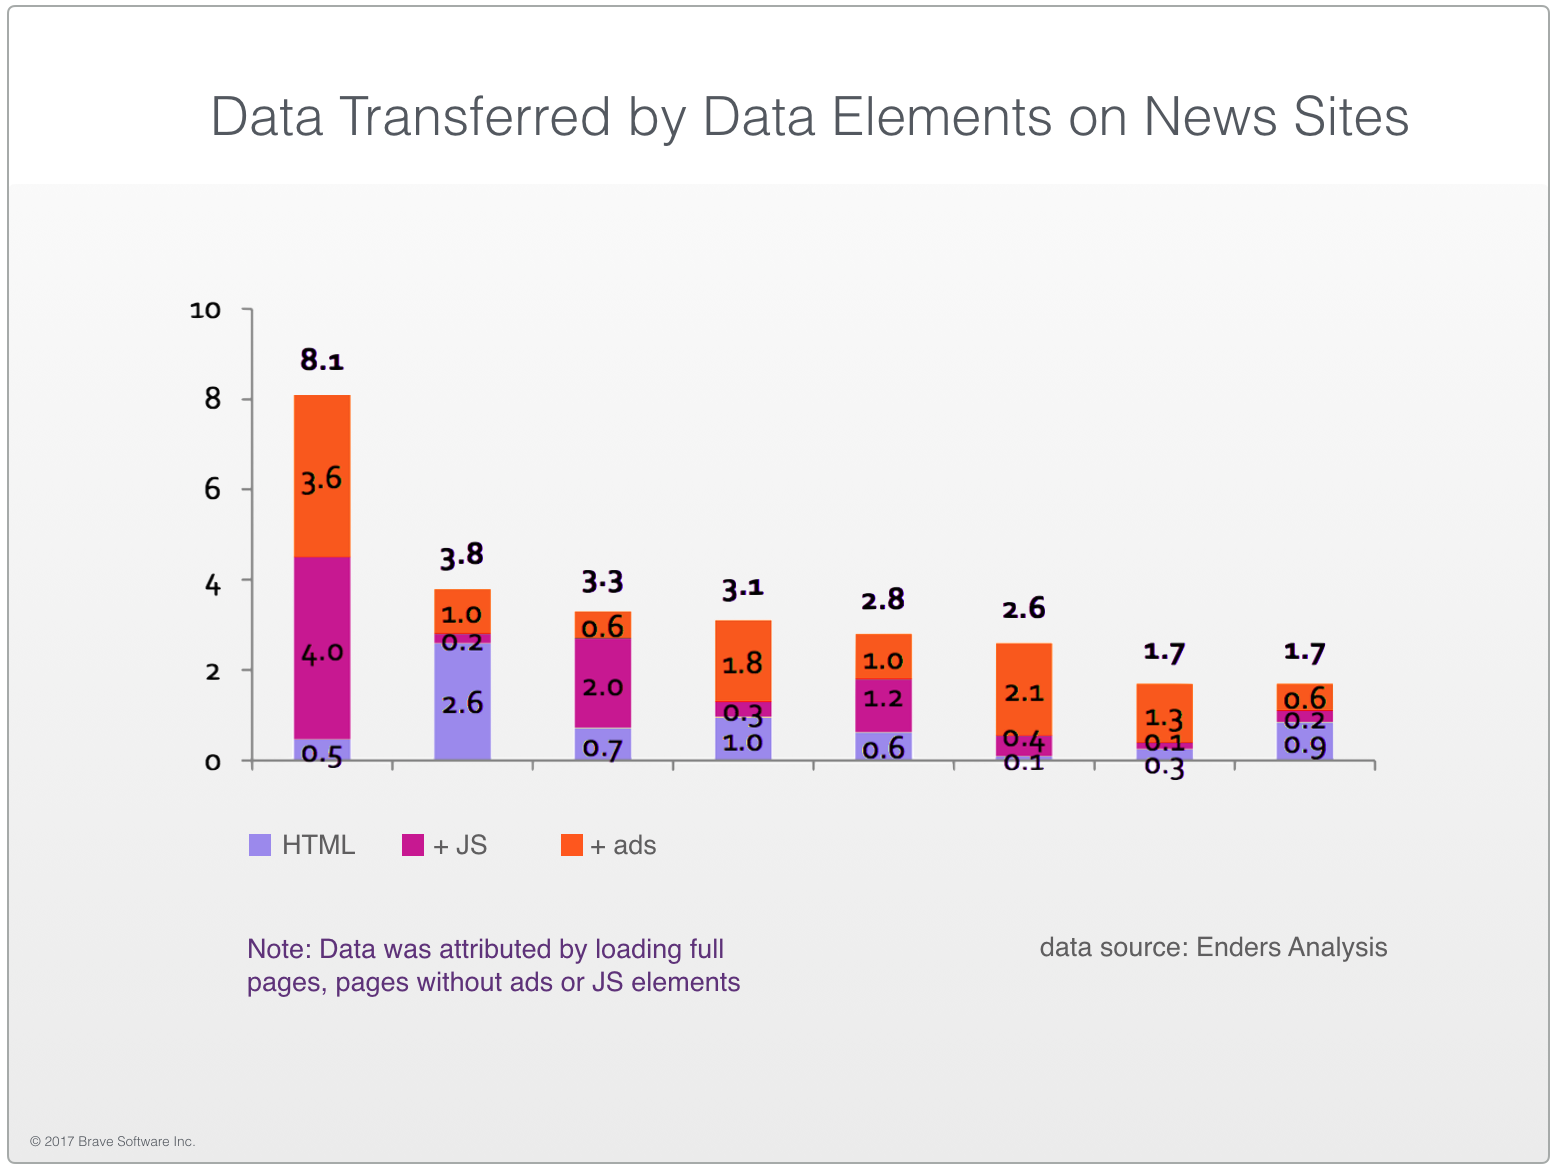
\includegraphics[width=0.9\textwidth]{data_transfer_news_sites.png}
\caption{Data Transferred by Data Elements on News Sites}
\end{center}
\end{figure}



Advertisers face fraud, while users are increasingly encountering malvertisements. Malvertisements are fake ads that trick users into clicking on them and then downloading malicious code, including ransomware. They can also entice users to visit fake domains used to steal financial information. According to a RiskIQ report released last year, “malvertising advert rates [rose] by 132\% from 2015 to 2016.” The sites most frequently hit by malvertising, according to Bromium\cite{8}, are news and entertainment sites. 



\begin{figure}
\begin{center}
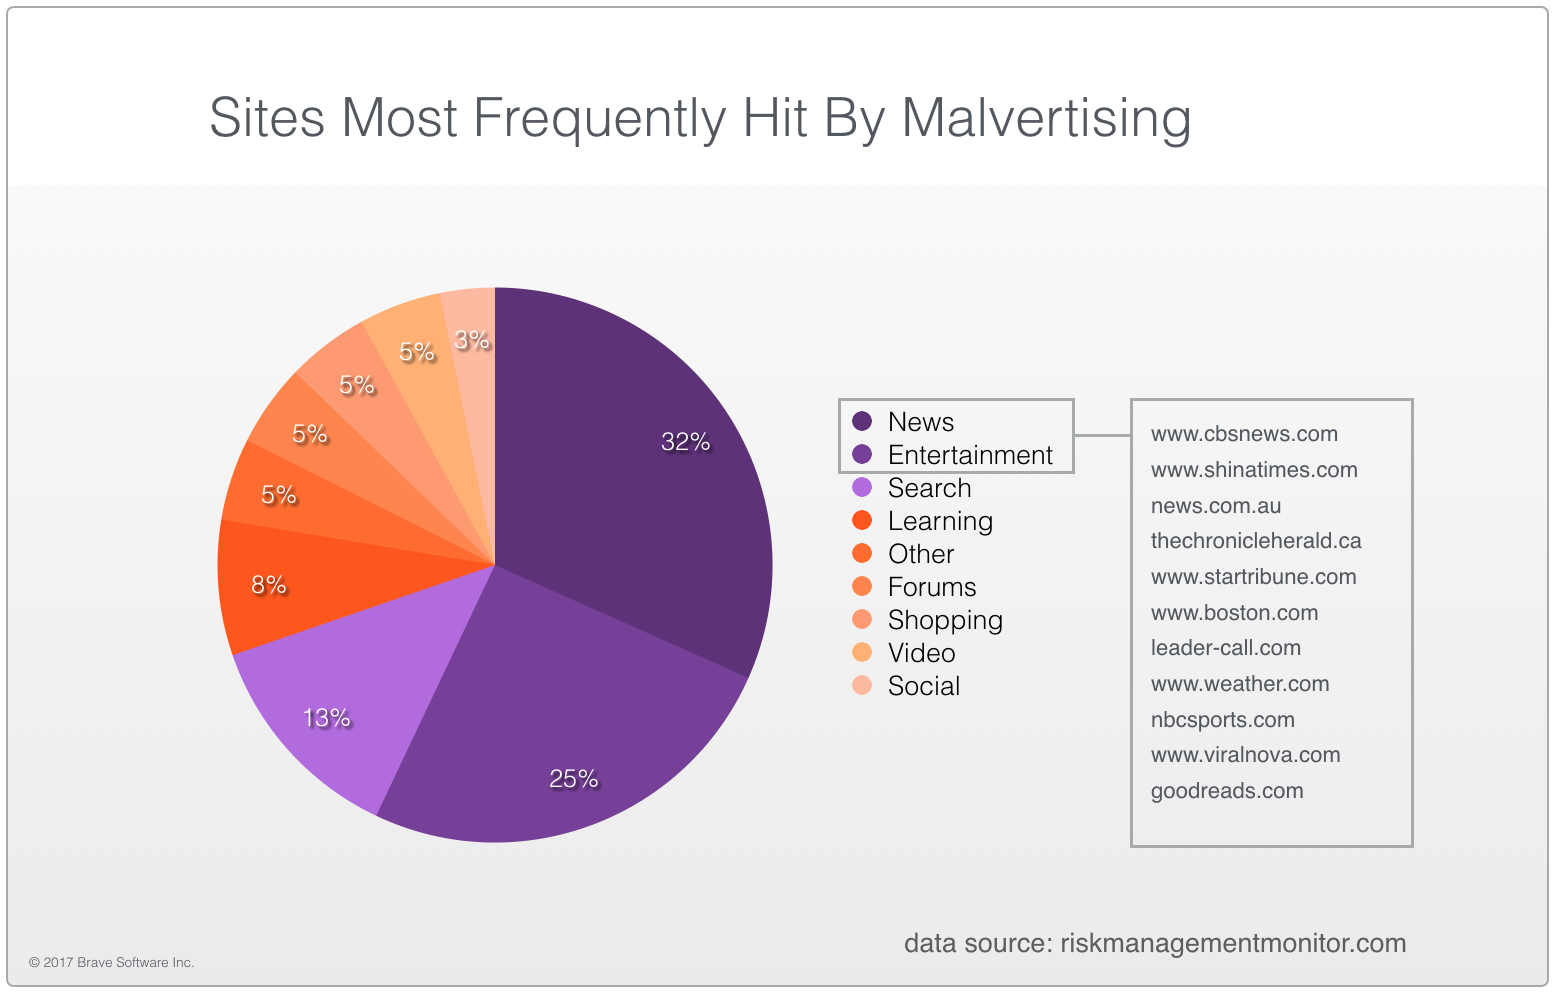
\includegraphics[width=0.9\textwidth]{hitbymalvertising.png}
\caption{Sites Most Frequently Hit By Malvertising}
\end{center}
\end{figure}


Web users are also not fully aware of the costs they pay for privilege of seeing advertisements. According to Business Intelligence, one study found that up to 79\% of mobile data transferred during visits to “popular publishers” was a result of ads. “The researchers compared data usage when a full page loaded without an ad blocker, with an ad blocker, and with an ad blocker and JavaScript disabled:”


The article noted that the researchers concluded that “advertising accounts for half of all the data used by publisher pages loaded over mobile data networks” during the tests. The average smartphone user consumes 1.8GB a month. Based on carrier plans for 2Gb, this means that users end up paying approximately \$23 a month to download ads, trackers, scripts and other related data.\cite{9}


\begin{figure}
\begin{center}
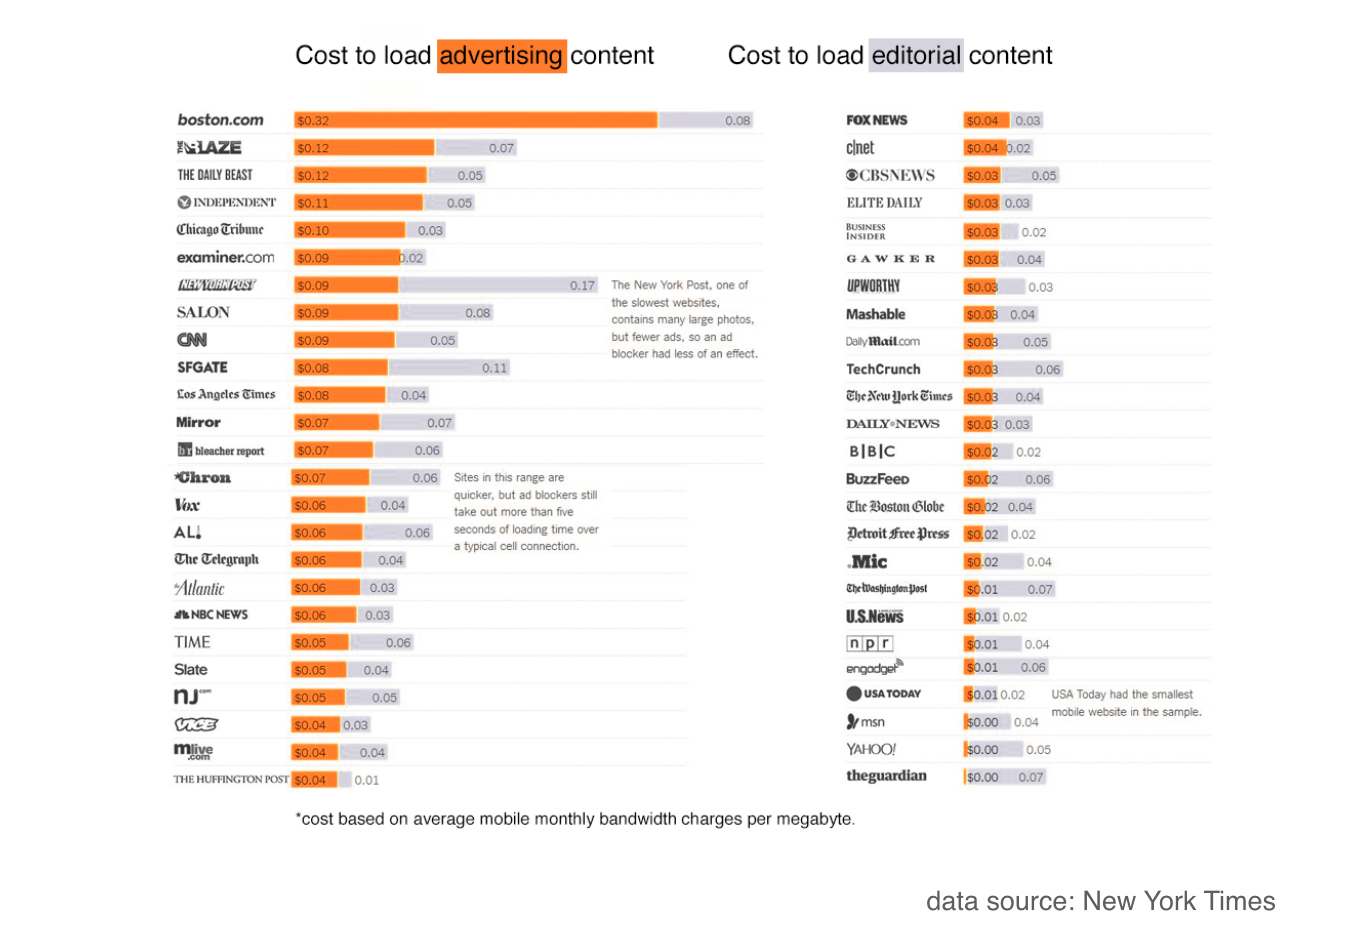
\includegraphics[width=0.9\textwidth]{cost_to_load_ads.png}
\caption{Content Loading Cost Comparison}
\end{center}
\end{figure}


A similar study by the New York Times found the data used by advertising resulted in significant  download times and costs across 50 top publishing sites. On one extreme, \href{https://www.boston.com}{www.boston.com} took 30.8 seconds for advertising and 8.2 seconds for editorial. The article concluded that removing ads saved “more than five seconds of loading time over a typical cell connection” for the articles studied. The data to load the ads came with a financial cost as well -- the price for the advertising content often outweighs that of editorial material:

The sum total of malvertisements, load times, data costs, battery life, and privacy loss has driven users to adopt ad-blocking software. This only further reduces publisher revenues and leaves the remaining ad-viewing audience even harder to target.

Ad blockers are a growing problem for publishers. Studies confirm that users of ad blocking software prefer the simplicity of navigation of ad-free or nearly ad-free content. Users of ad blocking software want to favor the content they value with their attention without distractions.  


\begin{figure}
\begin{center}
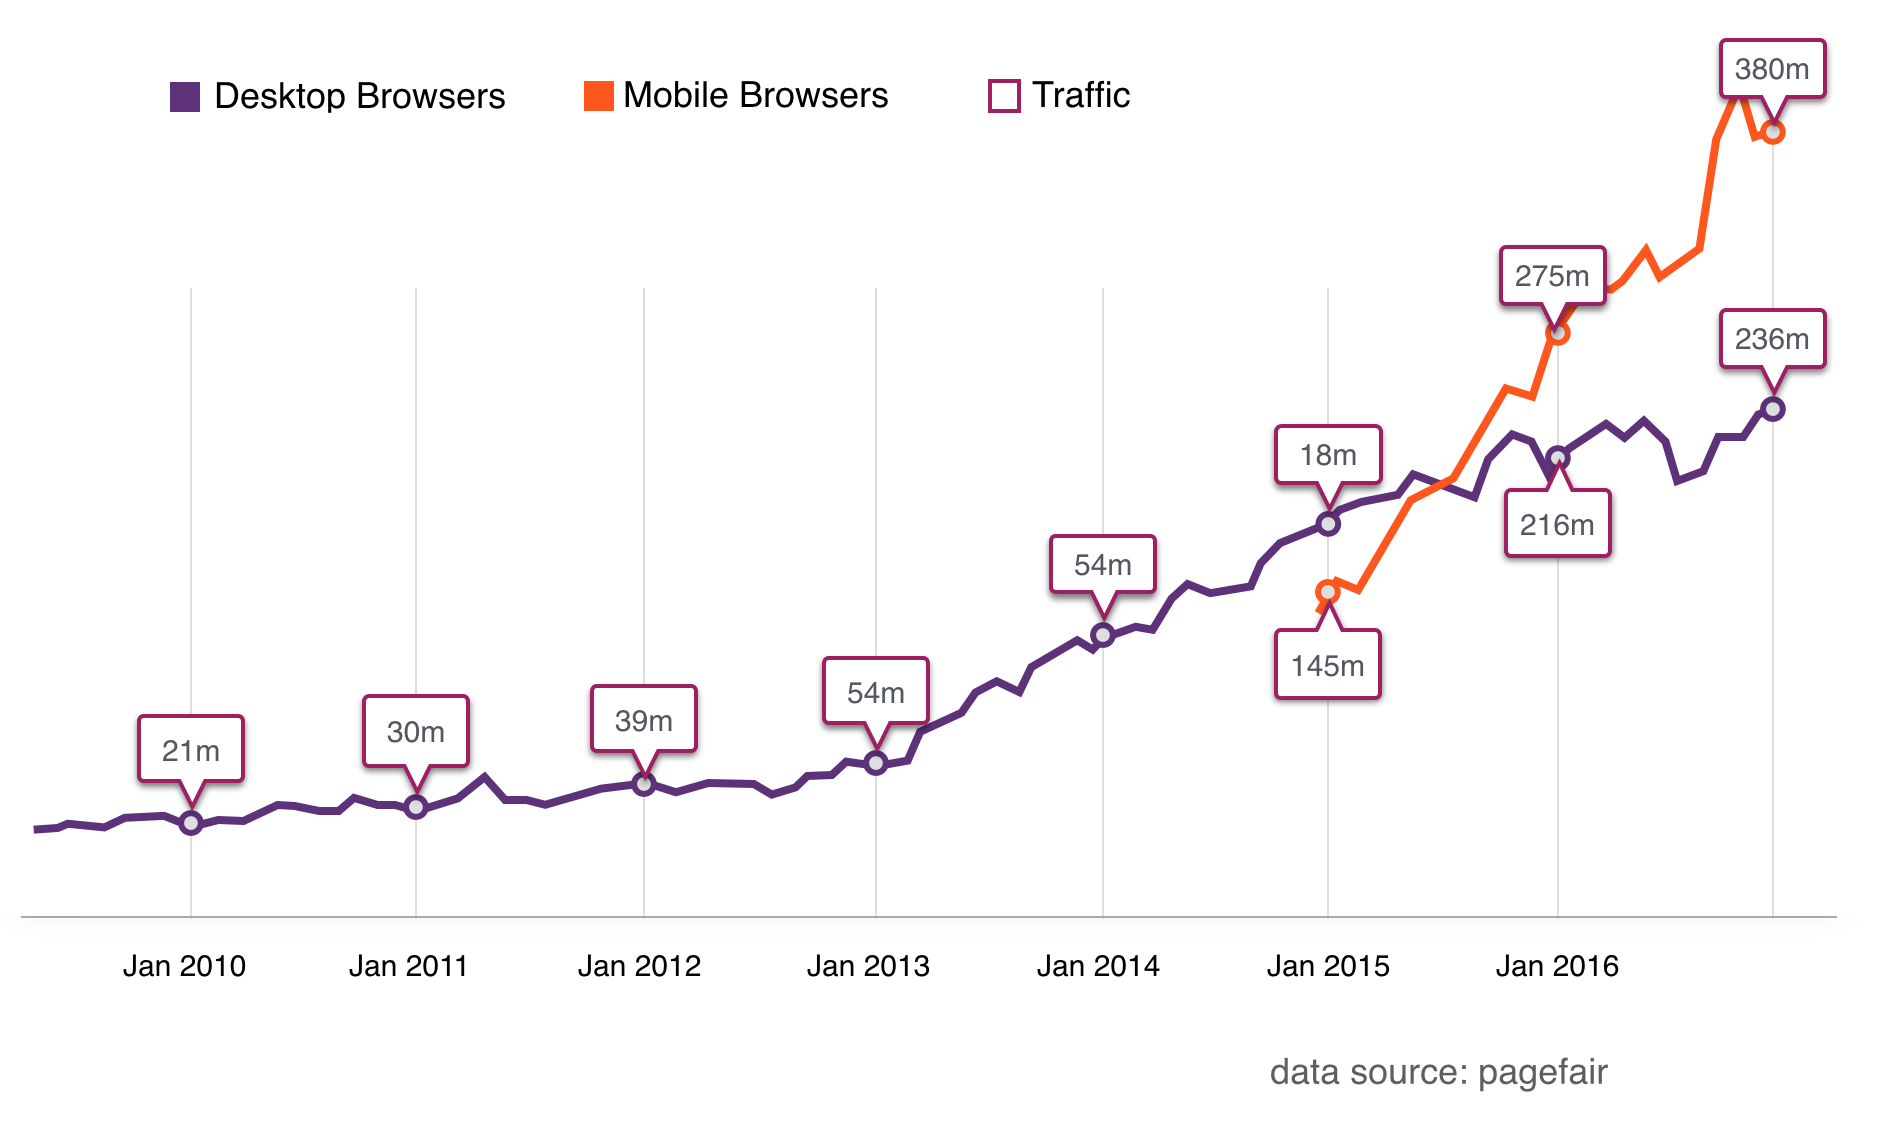
\includegraphics[width=0.9\textwidth]{adblock_growth_by_device.png}
\caption{Ad Blocker Growth by Device}
\end{center}
\end{figure}

It is projected that 86.6M Americans will use an ad blocker in 2017\cite{10}. Younger users are also more likely to adopt ad blocking technology, making the long-term financial impact of this technology worse than it appears at first glance\cite{11}.



\begin{figure}
\begin{center}
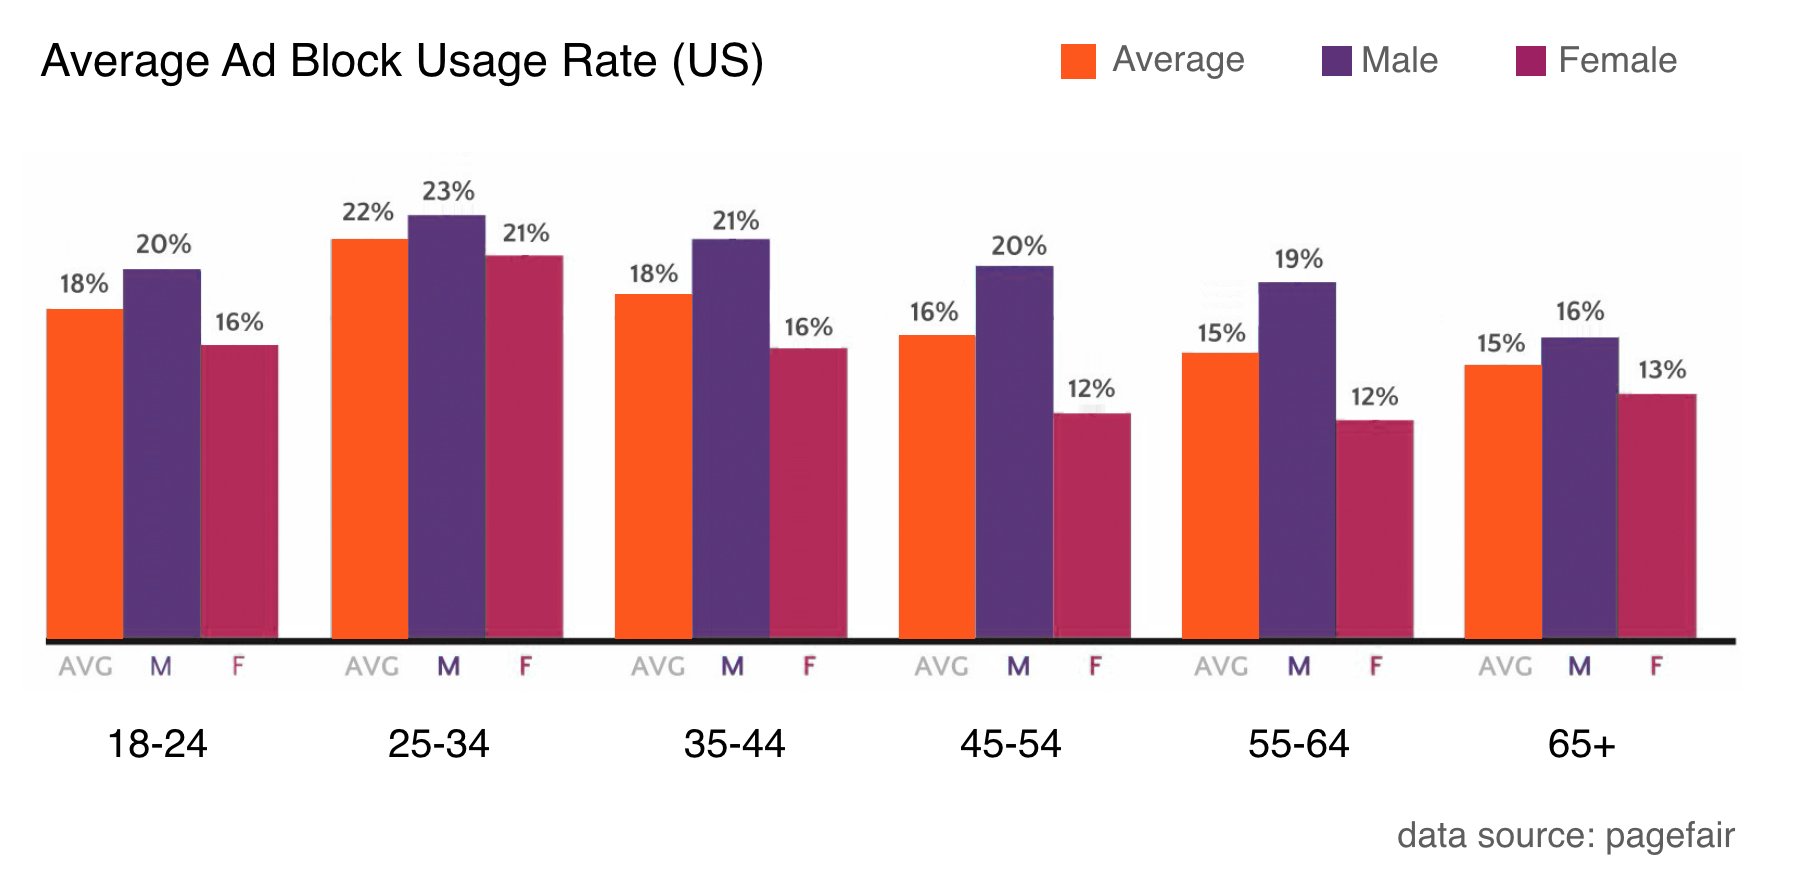
\includegraphics[width=0.9\textwidth]{adblock_usage_demographics.png}
\caption{Demographics of Ad Blocker Usage}
\end{center}
\end{figure}



This “perfect storm” for publishers has only gotten worse over the last few years as Google and Facebook have taken more and more share of advertising revenues. Together they claim \textit{over 73\% of online digital ad revenue, and an astounding 99\% of all growth from 2015 to 2016 in US total online ad budget}\cite{12}.
The increased attention for publishers brought by Google and Facebook would seem to be a net positive. But the traffic driven by social media is of lower quality than direct links. Users who arrive at a news site from social media typically only engage with the site for a third\cite{SocMed} of the time compared to those who are direct visitors. Distributed content hosting makes up only 14\% of publisher revenues, with the majority of the revenue coming from Youtube\cite{DCN}; many publishers have experienced serious commodification problems with these platforms.


\begin{figure}
\begin{center}
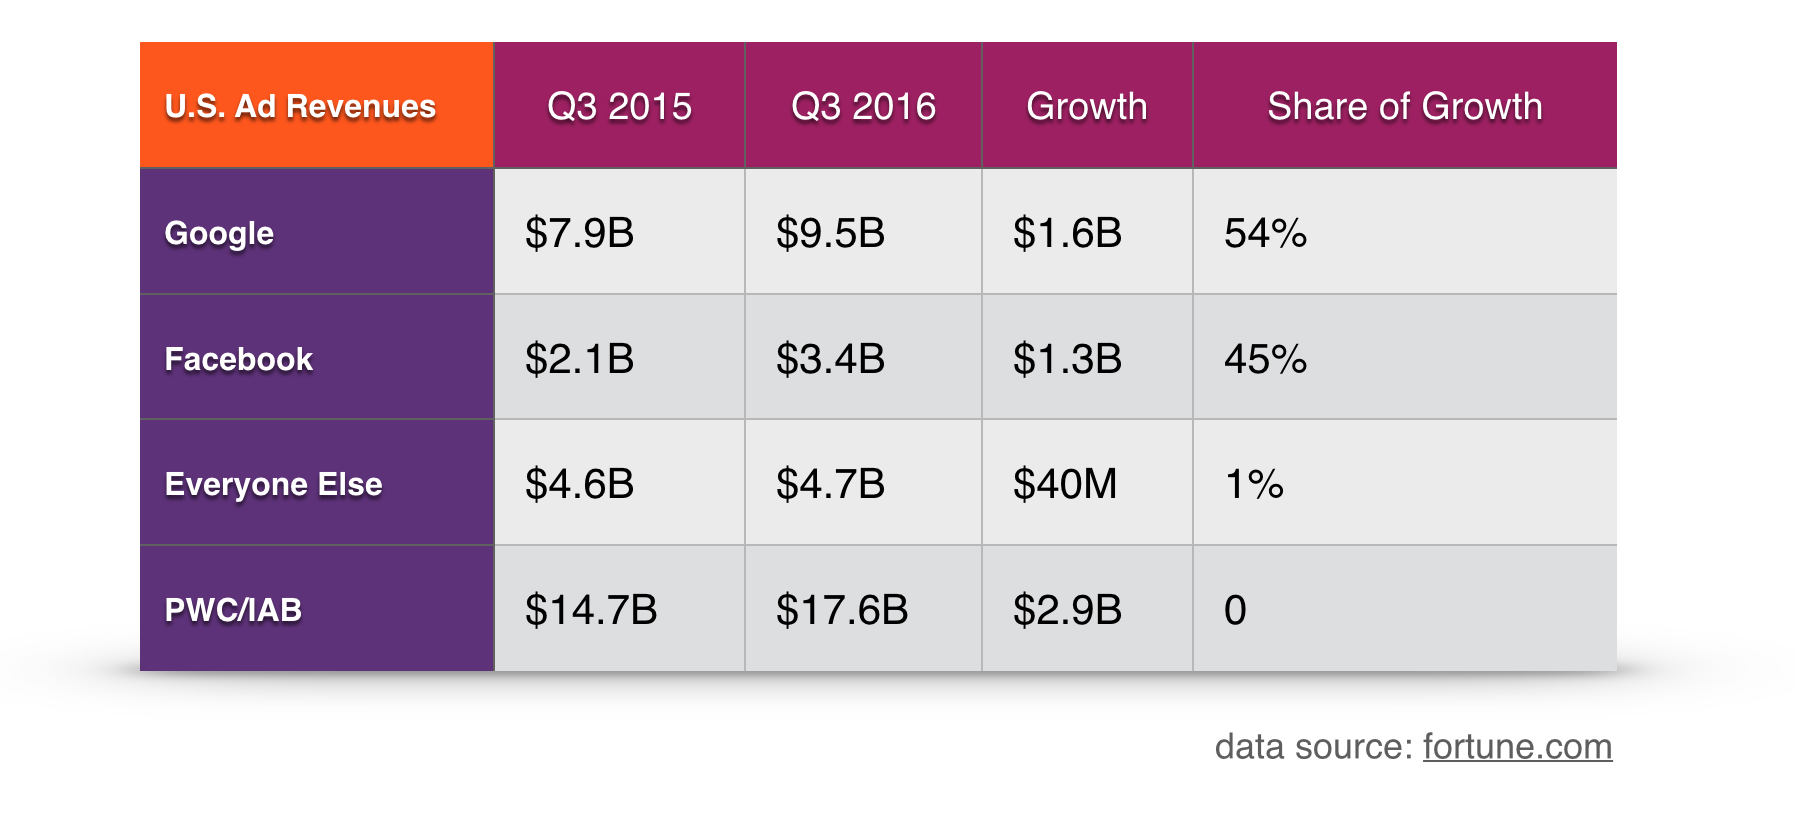
\includegraphics[width=0.9\textwidth]{google_FB_everyone.png}
\caption{Ad Revenue for Google vs Facebook vs Others}
\end{center}
\end{figure}



Advertisers on these platforms also face serious challenges. The sheer size of the platforms make for extreme non-transparency in assessing effectiveness of the advertising campaigns they host. Since most of the analytics products targeting these platforms are provided by the platform owner, principal-agent conflicts arise. Some advertisers have decided that traffic coming from the walled gardens isn’t worth the trouble. Some have even suggested based on third party analytics that a large proportion of the traffic is without value to the advertiser\cite{WithoutValue}.

In an effort to expand their walled gardens and to reinforce market dominance by traffic and data otherwise ingested from users directly on the publisher domain, major platform players have begun offering alternative content delivery channels with claims of incentivized placement and a faster, more secure user experience. While Facebook Instant Articles, Google AMP project and Apple News delivery channels were initially presented to publishers as opportunities to extend reach and visibility, they ultimately diminish publishers’ control of their brand narratives and reader relationships, and divert direct attention away from publisher sites over the long run.


\begin{figure}
\begin{center}
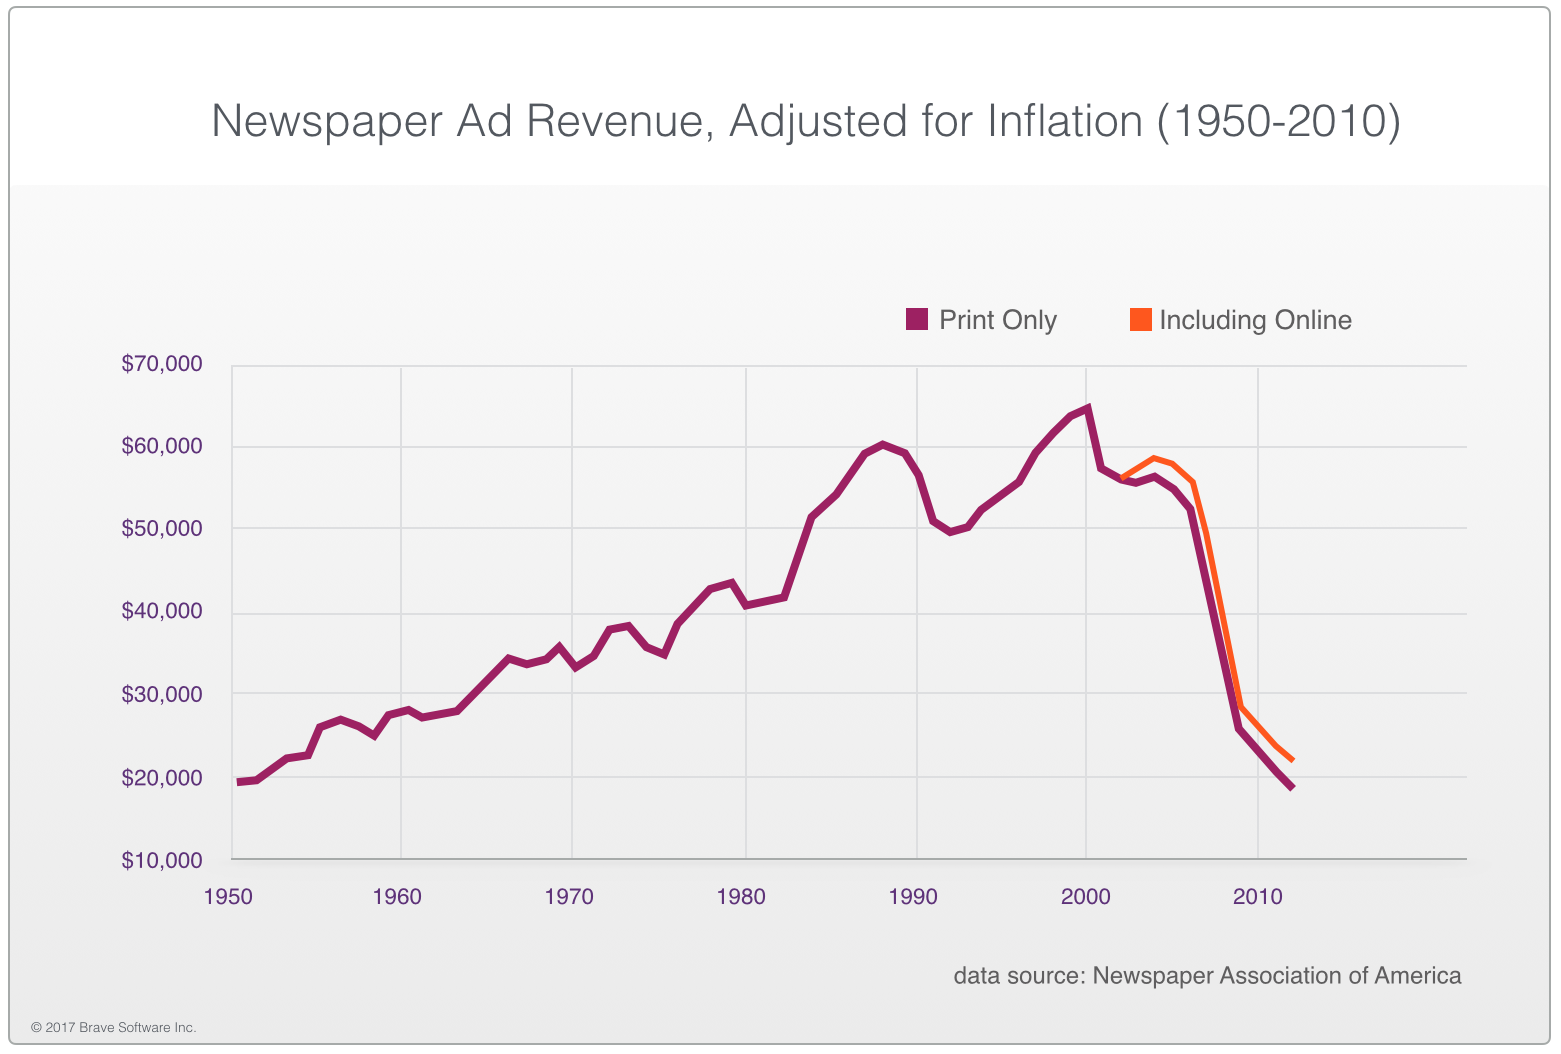
\includegraphics[width=0.9\textwidth]{newspaperadrev.png}
\caption{The Fall of Newspaper Ad Revenue}
\end{center}
\end{figure}


The publishing industry faces an existential threat. Legacy publishers have faced declining revenues for decades. Pressures on publishers to create content optimized for clicks has resulted in cut-backs to long form articles, investigative journalism, and foreign news bureaus, and has spawned the much lamented social cost revealingly named “clickbait.” The advent of ad blocking technologies portends catastrophic outcomes for modern publishers.
This dysfunctional dynamic has been noticed across the industry. Marketing budgets continue to climb\cite{Gartner1}, yet publisher revenues are static or shrinking\cite{Econsul}. This indicates serious market inefficiencies which can be repaired with a simplified and more efficient economic system based on new technologies.

\section{A New Deal: Attention-based Economics on Blockchain}
\label{sec-4}

The diversity of middle-men and the lack of value-add to the publisher and user make some sort of simplification of the present online advertising ecosystem inevitable. Present trends are toward an oligopoly where gatekeeper companies such as Google and Facebook control the entire online marketing budget with publishers powerless to control their revenues. Also, as users continue to adopt ad blocking technology the consequent shrinking of the remaining ad-funded market seems inevitable. 

The reality remains: user attention is valuable, but it hasn’t been properly priced with an efficient and transparent market system. While it has become a platitude that vast amounts of information are generated on and by the Internet, human beings are only able to devote a limited amount of attention to certain small subsets of the information. Information in the modern age is relatively cheap. Human attention paid to the information is the rare quantity. As Herbert Simon put it in an influential 1971 article:

\begin{quote}
\textit{``\ldots{}in an information-rich world, the wealth of information means a dearth of something else: a scarcity of whatever it is that information consumes. What information consumes is rather obvious: it consumes the attention of its recipients. Hence a wealth of information creates a poverty of attention and a need to allocate that attention efficiently among the overabundance of information sources that might consume it.''}
\end{quote}

Ultimately, a publisher provides information which may be of value to the user. Users give attention to the publisher in return for information that they value with their attention. At present, the publisher is paid by monetizing attention via a complex network of intermediary players through ad networks and other such tools. The publisher isn't paid proportionally to the attention given by the user. The publisher is actually paid proportionately to the indirectly measured attention given by users to ads. Publishers are used to working with this model for print ads, but web ads remain problematic for many of the reasons stated above. Users are subjected to the negative externalities that come with the present advertising ecosystem.

Users thus suffer a form of “electronic pollution” consisting of threats to security, threats to privacy, costs in inefficient download times, financial costs in extra mobile data fees, and in the case of the many ads, excessive costs to their attention. Human attention can be exhausted, until dopamine levels recover. Neurons can and do learn to ignore ad slots (so-called “banner blindness”). Abuse of user attention and permanent loss of users, via ad-slot blindness and ad-blocker adoption, make attention different from substitutable commodities such as pork bellies or crude oil, in the final analysis. While most users may be willing to pay some price for access to the publisher’s information, user attention is mispriced when we sum up the growing negative externalities imposed by the present advertising ecosystem.

\subsection{Basic Attention Metrics}
\label{sec-4-1}

The ability to anonymously monitor at the browser allows for the development of rich metrics for measurement of user attention. For example it is known whether an impression has been served to an active tab, and measure the seconds of active user engagement.. A running count of content viewed can be kept in a moving window, so if a user views some ad over some minimum threshold, a score could be constructed. Ads can also be anonymously matched with user interests using local machine learning algorithms to judge the content to which the user is paying attention. Several scoring algorithms have been tried with the Brave donation \href{https://github.com/brave/ledger-client}{ledger system}, which automatically donates an amount proportional to the attention given to a website. 

One of the metrics suggested is 5 total views of advertising content in an active window, for at least 5 seconds each. Hits of this nature would be calculated on a 30 day moving window. 

Another suggested metric is the “concave” score. This is a score which rewards a publisher for a thresholded and bounded function of the amount of time spent with the open and active page.  For example, one “point” could be awarded for a two second view of the page, with two points for a 30 second view, and 3 for a 60 second view, with diminishing or bounded returns for longer views.

The present implementation of the concave score, which is being used to distribute attention metered donations to the publishers us a thresholded, time limited quadratic score. The formula is as follows:

\[ score= \frac{-b + \sqrt{b^2 + 4a*duration}}{2a}\]

where where $a=13000$, $b=11000 $ and $duration$ is measured in
milliseconds. This gives a minimum threshold of 25 seconds to achieve
a score of 1. The upper bound is set to be around 12 minutes of
attention given to the article, with a maximum score for a given piece
of content of 7. 

The plot of the BAM as presently implemented:


\begin{figure}
\begin{center}
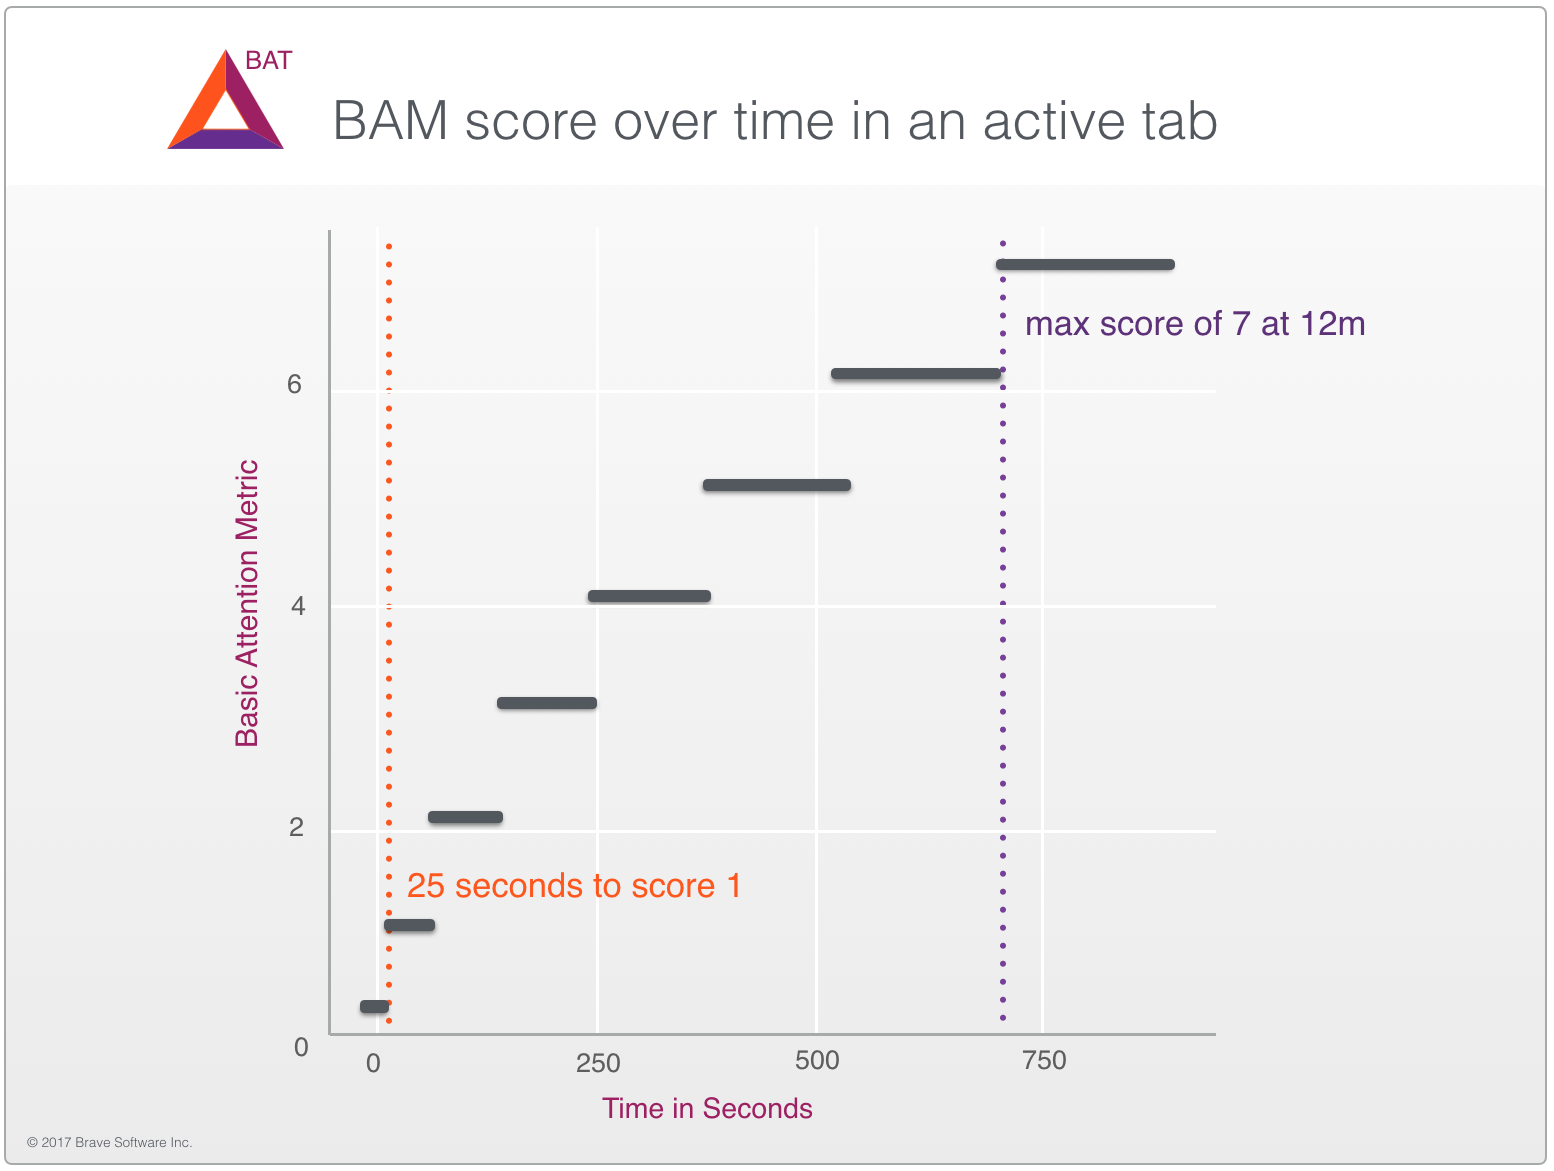
\includegraphics[width=0.9\textwidth]{BAM_score_over_time.png}
\caption{Basic Attention Metric Score Over Time}
\end{center}
\end{figure}


Another potential metric is a targeted ad based on a subset of keywords purchased at the advertising partner end, combined with the attention metric, essentially selling the attention along with an advertising topic. 

We expect publishers and advertisers to suggest new metrics of user attention to be surfaced, and encourage other vendors to build on the topic as we progress.
\subsection{Token Technology}
\label{sec-4-2}

The Basic Attention Token (BAT), a token based on the Ethereum technology, is an important element of a new marketplace. Ethereum is an open source, blockchain-based distributed computing platform oriented towards smart contracts. Effectively the Ethereum technology is a distributed virtual machine that allows end users to construct smart contracts for transactions. Smart contracts are stateful applications stored in the Ethereum blockchain. These contracts are cryptographically secure and can verify or enforce performance of the contract. Token contracts are a standard feature of the Ethereum ecosystem.

Ethereum technology has been used for mobile payment systems, distributed exchanges, tokens pegged to commodities and fiat currencies, market clearing mechanisms, micropayment systems for distributed computing resources, commodities and securities exchanges, crowdfunding, and legal document verification. Large firms have invested in and deployed the Ethereum technology, with JP Morgan, Deloitte, IBM, Santander Bank, Microsoft, the Luxembourg Stock Exchange, and the Royal Bank of Scotland being key early adopters.

Micropayments using BAT will be accomplished for the first stage deployment with the Brave Micropayments \href{https://github.com/brave/ledger}{Ledger}. Each viewed ad will be verified at the browser using the BAM. 


\begin{figure}
\begin{center}
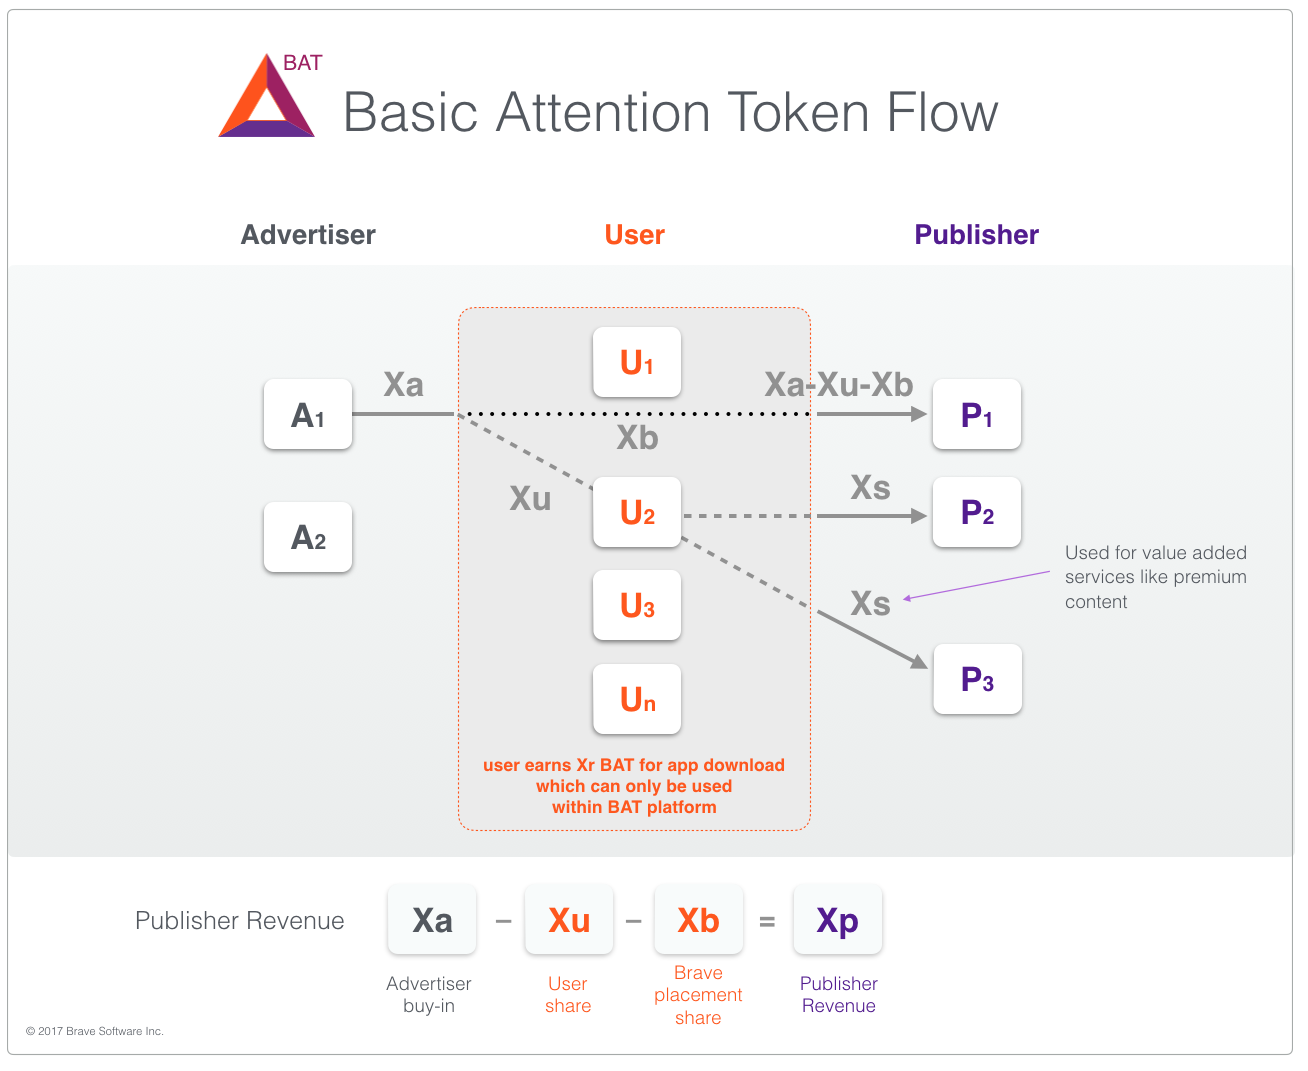
\includegraphics[width=0.9\textwidth]{BAT_tokentech_diagram.png}
\caption{Value Flow of the Basic Attention Token}
\end{center}
\end{figure}



This flow shows the conceptual flow of the BAT payments. The flow of the BAT payments will not follow this chart precisely in first iterations of the BAT payment system as the payments will be regulated by the Brave ledger system, but the total effect will be the same. The high level concept is the advertiser sends a payment in token along with ads to users in a locked state Xa. As the users view the ads, the flow of payments unlocks, keeping part of the payment for their own wallet (Xu), and passing on shares of the payment to brave (Xb) and passing the remainder on to the Publisher (Xa-Xu-Xb).  

The BAT will, in early stages, be specifically tied to Brave browsers and Brave servers, along with verified publishers. Ad fraud will be prevented by publication of source code and cryptographically secure transactions. Ads served to individual browser/users will also be rate-limited and tied to active windows and tabs. Payments in BAT will be sent only to publishers, though a payment for viewing an ad on one publisher may be used at another publisher or kept for some other premium services supplied through the BAT system.

\subsection{Tokens Used as Publisher Payment}
\label{sec-4-3}

Publisher payment will be through the BAT system. For the first deployment of BAT, the transactions in BAT will take place through the Brave Ledger system, which is an open source zero knowledge proof scheme presently deployed to allow Brave users to make anonymous donations to publishers using bitcoin as the medium of exchange.  The Brave Ledger system uses the ANONIZE\cite{13} algorithm to protect user privacy. 

For the first incarnation of BAT, all payments in BAT must have a publisher endpoint. The \href{https://github.com/brave/ledger-publisher}{publisher client} as it is coded today already measures user attention as described above. The “concave” awarding mechanism calculates an attention score based on a fixed threshold value for opening and viewing the page for a minimum of 25 seconds, and a bounded score for the amount of time spent on the page. A synopsis of user behavior is then sent back to the Brave Ledger System for recording and payments made on the basis of the scores.

Much of the infrastructure required to deploy BAT at the back end is presently “code complete,” in place and being used to distribute donations based on user attention. As such, this infrastructure will be leveraged to deploy BAT as soon as possible for testing, user, and advertiser feedback.

A fully distributed ledger is desirable, both for public accountability and potential scalability reasons. Publishers, advertisers and users of the BAT token will have incentive to use such a system to keep track of payments within the BAT system. 

State channels allow for multiple small transactions with strong anonymity guarantees when using the correct matching algorithms. While Raiden and ZCash are new state channel schemes becoming integrated with the Ethereum ecosystem, it is likely that a new scheme addressing the unique problems of this type of transaction will be used for large scale multiparty transfer of BAT.
 A lottery system may be used, where small payments are made probabilistically, with payments happening essentially in the same way that coin mining works with proof of attention instead of proof of work\cite{14,15}, BOLT\cite{16}, Zero knowledge SNARK\cite{17} or STARK\cite{18} algorithms may become part of this stack for guarding privacy of participants. The BAT situation is mitigated by the fact that only the privacy of the browser user is important; publishers and advertisers have no privacy concerns and may even prefer to put their information on a public ledger for settlement purposes. The transactions in a fully distributed BAT system will almost always be one to many and many to one, therefore novel zero-knowledge transactions may be suggested by this arrangement.

As Brave moves to a fully distributed micropayment system, we expect other developers to use our free and open source infrastructure to develop their own use cases for BAT. We want BAT and the tools associated with it to eventually become important web standards for future development of web content. Publishers, advertisers and users who view web content deserve a private, secure and well engineered future.
\subsection{Tokens for User Applications}
\label{sec-4-4}

As users are given access to some of the advertising spend in BAT, they will become an important and active part of the advertising and publishing economy, rather than the passive participants they are presently treated as. While tokens can be donated to individual content providers and publishers, there are any number of use cases for the tokens.

A very obvious use case is for very specific targeted advertising. Many small businesspeople have modest requirements which may be well served by tokens they acquire through their normal browsing activities. Users may also find new uses with low barrier to entry highly targeted ads; personal ads targeting people of a religion or subculture for example.

Some publishers may have premium content they would ordinarily only offer to subscribers. Since subscription models are not typically favored by users on the internet, this could unlock new revenue for premium content providers. Content may also be bought for friends using the token; if someone likes a premium article, they can make a micropayment to send it to three of their friends.

Higher quality content may also be offered to users for a BAT transaction. For example, higher quality video or audio on an entertainment channel, or some kind of summary of headlines in a news source. Video or audio content in a news or other information source may be restricted to people who pay a small micropayment.

Comments may be ranked or voted on using BAT tokens, similar to the “thumbsup/thumbsdown” on some comment sections. Comment votes backed by BAT may be given more credibility due to the fact that someone cared enough to back the comment with what would be a limited supply of token, as well as the fact that a token transfer can be verified as coming from real people rather than robots. The right to post comments may also be purchased for some minimal payment, to cut down on abusive commenters.


\subsection{Roadmap}
\label{sec-4-5}
\begin{itemize}
\item{Pre 1.0 Brave already has an anonymized ledger system for making donations and payments to publishers based on user attention. The secure vault using the ANONYZE algorithm to ensure customer privacy is an important piece of the BAT ecosystem which is already in place and deployed in Brave. Brave is already measuring user attention at the browser and distributing donations to the publishers using this system.}
\item{1.0 BAT: BAT wallet integrated with the Brave browser. Verification and transactions to be handled by Brave’s internal zero knowledge proof ledger system to protect individual user anonymity from advertisers, publishers and third parties. The ads will be bought and sold based on the first version of the Basic Attention Metric (BAM). }
\item{Beyond 1.0 BAT: Make the transfer and verification process entirely distributed on Ethereum using a state channel scheme with zero knowledge proof protocol for ensuring user privacy. Add alternate BAM metrics based on advertiser feedback. This will allow for full user privacy as well as a decentralized audit trail for advertisers, users and publishers to ensure they received correct payments for the advertising delivered through the BAT network.}
\item{Browser as platform/BAT:  Further BAM metrics based on advertiser feedback as needed. Partners building applications on the BAT infrastructure. Also, at this point we plan to explore value-added services that can be offered to users on the browser platform through BAT.}
\end{itemize}


\section{Business landscape}
\label{sec-5}
\subsection{Competition}
\label{sec-5-1}
\begin{itemize}
\item{Reddit Gold is a premium membership program, granting access to extra features to improve experience. Reddit is a major publisher, but this program is designed by to and limited to Reddit. It does not offer publishers a mechanism for publishers and users to monetize through the use of Blockchain-based token.}
\item{Steem is social-media and blogging platform lets users earn revenue when they receive upvotes. It is a kind of monetized Reddit. Steem does use Blockchain, but it is not a generalized means for publishers and users to be rewarded for content. In short, it is not a Blockchain-based digital ad platform. It is specific to the Steem platform. }
\item{Blendle is a kind of iTunes for journalism, offering micropayments on a per-story basis. It gives  readers a collection of stories based on preferences. Brave and BAT do not curate anything. Users merely go about their business on the web and publishers are rewarded. Blendle is not a token-based digital advertising platform. }
\item{Google is a search engine company that makes most of its revenue from digital advertising. Google is at the center of the existing digital advertising ecosystem. They benefit from the complexity and opaqueness that defines it. BAT intends to empower the very users and publishers that are receiving less than they should. Google does not have a Blockchain-based tokenized system of offering rewards. Users are often unaware of how their privacy is compromised using Google.}
\end{itemize}

\subsection{BAT Advantage Matrix}
\label{sec-5-2}

\begin{tabu}  to  \textwidth {|c|c|} \hline

{\textbf{Present ecosystem}} & {\textbf{BAT token ad payments}} \\  \hline

User frustration over loading time & Fast loads\\ %\hline
Walled gardens & Free software, open source infrastructure\\ %\hline
Bandwidth wasted & Low bandwidth overhead\\ %\hline
Screen clutter & Uncluttered screen \\ %\hline
Irrelevant ads & Ads tuned to user interests \\ %\hline
Security issues & No malware \\ %\hline
Viewability problems/attribution & Secure attribution/attention score\\ %\hline
Advertiser uncertainty about delivery & Perfect delivery certainty \\ %\hline
CPM/click based & Attention-based \\ %\hline
Reader attention not valued & Reader is paid for attention \\ %\hline
Publisher revenues lowering & Larger publisher revenues \\ %\hline
Expensive ad buys due to middlemen & Efficient ad buys \\ %\hline
Complex/expensive viewability metrics & Simple/free viewability metric \\ %\hline
User’s privacy violated & Perfect user privacy \\ \hline
\end{tabu}


\subsection{Brave Overview}
\label{sec-5-3}

Brave (\href{https://brave.com/}{https://brave.com/}) is a fast, open source, privacy-focused browser that blocks invasive ads and trackers.

Brave is more than a browser: it defends your data on your devices and synchronizes your personal and private browsing profile across devices using client-side encryption. Your data, studied and abstracted by on-device-only machine learning, provides you with private and anonymous options to get compensated for your attention. Brave cuts out all third party trackers and middle-players, eliminating data leakage, malvertising risk, and excessive fee-taking. Brave does this while providing publishers with a substantially larger revenue share than they are receiving in existing inefficient and opaque marketplace. 

Brave thus aims to reset the online ad-based Web ecosystem, giving advertisers, publishers and users a win-win solution whose components and protocols can become future Web standards. 
\subsection{Key Team Members}
\label{sec-5-4}
\begin{itemize}
\item{\href{https://www.linkedin.com/in/brendaneich}{Brendan Eich}, CEO, co-founded Brave. Previously, he co-founded Mozilla and Firefox; he is the creator of JavaScript.}
\item{\href{https://www.linkedin.com/in/bbondy/}{Brian Bondy}, Lead Developer, co-founded Brave. Previously, he was at Khan Academy, Mozilla, and Evernote.}
\item{\href{https://www.linkedin.com/in/richterbrad/}{Bradley Richter}, Head of Design, was previously at  EFI, Fiery, eBeam and a co-founder of Luida.}
\item{\href{https://www.linkedin.com/in/brian-johnson-aaa11018/}{Brian Johnson}, Senior Engineer, was previously at JD Power and Korrelate.}
\item{\href{https://www.linkedin.com/in/yan-zhu-b7124227/}{Yan Zhu}, Senior Engineer, is an EFF Fellow and was previously at Yahoo. She has contributed to the TOR Project, HTTPS Everywhere, and Privacy Badger. Named as one of \href{https://www.forbes.com/sites/bruceupbin/2015/01/05/meet-the-30-under-30-rising-stars-in-enterprise-technology/}{Forbes’ 30 under 30} Rising Stars of Enterprise Technology in 2015.}
\item{\href{https://www.linkedin.com/in/marshallrose}{Marshall Rose}, Senior Engineer, PhD from UC Irvine, creator of SNMP and was with the Internet Engineering Task Force.}
\item{\href{https://www.linkedin.com/in/pureproductions/}{Luke Mulks}, Senior Ad-tech Specialist, for technical incident response, investigation, support \& issue resolution for ad tech and the Brave Browser. Developing/advising on ad tech and tracking threats that Brave shields users from (pr/blog).}
\end{itemize}

\section{Token Launch}
\label{sec-6}
\subsection{Token Launch summary}
\label{sec-6-1}
\begin{itemize}
\item{Maximum financing: 800,000 ETH}
\item{Minimum financing:  200,000 ETH}
\item{1 ETH = 1,000 Basic Attention Tokens (BAT)}
\item{Token contract address: TBD (Published through various channels 24hrs before launch date)}
\item{Launch date and time: TBD}
\item{Token launch time-frame: 30 days}
\item{Token launch completion: Token launch will end when either 800,000 ETH are raised or 30 days have expired. If less than 200,000 ETH are raised, ETH will be sent back to the sending address.}
\end{itemize}
\subsection{Token Distribution}
\label{sec-6-2}

At the end of the token launch, token will be released as follows:
\begin{itemize}
\item{Brave: 15\% (Locked for 6 months)}
\item{User growth pool: 15\%}
\item{Token available to public at launch: 70\% (corresponding to the ETH raised at token launch)}
\end{itemize}

\subsection{User Growth Pool}
\label{sec-6-3}
User growth fund is used to incentivize users to participate in the BAT ecosystem.
\begin{itemize}
\item{A 15\% endowment is for early adopters of Brave at 5 BAT/user}
\item{BAT received as a reward can only be used within the BAT ecosystem for value added services}
\item{Unused BAT after 6 months will be sent back to the user growth fund which can then be used for new users}
\item{Existing Brave users can get tokens by updating their app and verifying phone number}
\item{No new tokens will be created once the user growth pool is exhausted.}
\end{itemize}

\subsection{Budget Allocation}
\label{sec-6-4}
\begin{itemize}
\item{\textbf{Brave Team 60\% of budget:} The Brave team consists of just over 20 engineers. This financing allows for the rollout of the BAT solution, necessary adjustments to the existing Brave browser technology and the expansion of the user-base.  }
\item{\textbf{Administration 5\% of budget:} This consists of costs associated with running offices and personnel around the world. Brave is headquartered in San Francisco, has several employees in Canada and throughout the globe. This also covers legal, accounting, security audits, etc. }
\item{\textbf{Marketing 5\% of budget:} Marketing will focus on expanding awareness and adoption of the Brave browser and the BAT solution among users, publishers and advertisers. This also includes the growth and maintenance of the world-wide community. This is in addition to user growth fund.}
\item{\textbf{Contractors 20\% of budget:} These funds will be directed at third-party providers offering engineering, marketing, growth-hacking, PR, partnerships, affiliate programs and more. }
\item{\textbf{Contingency 10\% of budget:} This is a set-aside. }
\end{itemize}

\section{BAT FAQs}
\label{sec-7}


\textbf{What does BAT stand for and what is it? }\\
Basic Attention Token. The BAT, a token based on the Ethereum technology, is a unit of exhange in a new Blockchain based digital advertising system. User attention is anonymously monitored in the Brave browser and publishers are rewarded accordingly with BATs. Users also get a share of BATs for participating. \\
\\
\textbf{What do BATs represent?}\\
BATs are utility tokens in the Brave's Blockchain-based digital advertising platform. BAT tokens are not refundable. BATs are not securities, nor are they for speculative investment. BATs do not have or imply any promises of future performance or value. There is no promise of inherent value, no promise of continuing payments, and no promise or guarantee that BAT will hold any particular value. BATs do not represent and not any kind of participation in the company. BATs  hold no rights in the company. BAT tokens are sold as a functional good and all proceeds received by company may be spent freely by company absent any conditions. BATs are intended only for experts in dealing with cryptographic tokens and blockchain-based software systems.\\ 
\\
\textbf{How will Brave use ETH raised during token launch? }\\
The ETH received in the crowdsale will by used by Brave Software to build out the Blockchain-based digital advertising system, which uses BATs as a unit of exchange. Existing Brave investors will not receive any amount of ETH. For more information please check the budget allocation section in “Terms and Conditions.” \\
\\
\textbf{How will Brave store ETH? }\\
Brave will use a secure multisig wallet design similar to those used by Gnosis and Golem to hold the ETH. \\
\\
\textbf{Are BAT tokens transferable? }\\
After tokens have been released to participants in the token launch, then they can be transferred. Tokens used in the Browser may only be donated or used to pay publishers for premium content or for other services. Tokens may also be used by publishers  for promotions.\\
\\
\section{Appendix}
\label{sec-8}
\subsection{A More Efficient Market: Coase Theorem}
\label{sec-8-1}

Problems involving social and transactions costs have been studied by
economists. Ronald H. Coase was awarded the Nobel Prize in Economics
in 1991 for his work on the allocation of radio frequency resources.\cite{19}
Modern problems in ad-tech are addressable using the work of Coase and
subsequent commenters on his idea. At present, the effects of today’s
overcomplicated advertising ecosystem a negative externality or
“social cost” for the user. The user’s privacy is invaded, his
browsing experience compromised, and even his limited supply of
internet bandwidth on mobile devices is depleted by the present state
of this ecosystem. Effectively, the market for user attention has
become inefficient; the transaction costs of advertisers purchasing
attention have become too high. 

The widespread adoption of ad blocking technology adds a negative
externality on the publishers as well. If everyone blocked
advertisements, there would be little content left to exchange for
user attention, as publishers go out of business. An efficient market
for attention would remove these negative externalities, or compensate
all parties to the transaction in an efficient way. 

The Coase theorem states that trade in an externality or “social cost”
is possible. If there are sufficiently low transaction costs,
information symmetry, and well defined property rights, bargaining
will lead to a Pareto-efficient outcome regardless of the initial
allocation of property. 

The standard textbook example of the Coase theorem consists of a
factory which produces pollution as a side-effect of the manufacturing
process, and a neighboring landowner who suffers from the pollution. 

In the case where the neighbor owns the pollution rights;
  \[ Q= 1-(P + c) \]

$c$ is marginal cost of production, $P$ is price for pollution permit, $Q$ is marginal cost 
function for the manufacturer in the case. Neighbor has valuation $ \nu $ for clean environment,  and the sale of $Q$ pollution permits entails a loss of $ \nu Q = \nu(1-(P+c))$, so the neighbor finds the price of pollution permits by maximizing net benefit 

\[ \max_{P} \{ (1-(P+c))P - \nu(1-(P+c)) \} \]
The benefit maximization is \[1-2P -c + \nu = 0\]
Giving the price \[P =\frac{1-c+\nu}{2} \] and the units bought by the factory 
\[Q=\frac{1-c-\nu}{2} \]

   If the factory has the entire property right, the neighbor effectively purchases some share of the pollution right from the factory which it doesn't use. The neighbor wants to buy $Q=1-(P-\nu)$ units. The factory maximizes its net benefit with
   \[ \max_{P} \{ (1-(P-\nu))P - c(1-(P -nu)) \}  \]
   The factory's profit maximization is
   \[ 1-2P + \nu -c = 0\]
   So the price is still \[P=\frac{1-c+\nu}{2} \]

For Coase’s theorem to hold symmetrically, it requires well-defined
property rights. By definition, the user’s attention is the valued
quantity. The user can make the decision to block ads from a given
publisher, or choose to forgo interacting with a publisher altogether.

This makes it obvious that attention belongs to users de facto and
notwithstanding the efforts of some publishers and advertising firms
to assert ownership of user attention de jure. Even in commonplace
situations where user attention is de jure required, de facto, users
still own their own attention. For example, attention is required
while the safety demonstration is given on an airline flight, but
people often ignore it anyway.

Another requirement for validity of the symmetric version of Coase’s
theorem is information symmetry. Information asymmetry between
publishers, advertisers and users has kept the existing advertising
ecosystem in place for some time, but as we can see from the growing
use of ad-blockers, the information asymmetries on the user side are
crumbling. 

At present, advertisers and publishers have a severe information
asymmetry in that most of the metrics they use to assess campaign
effectiveness are indirect and administered by middlemen whose
interests are not aligned with the interests of one or both
parties. Complex “viewability” metrics create unnecessary conflict
between advertisers and publishers. There is no technical reason for
this information asymmetry; it can be mitigated with better
technology, in particular browser technology at the endpoint where all
the data can be measured privately and confirmed anonymously.

The final requirement, which is only a soft requirement for Coasean
analysis in the case of well-defined property rights, is that of low
transaction costs. The Coasean transaction cost refers to the cost of
negotiating a deal which can suit all parties to a dispute involving
social costs. With the existing ecosystem, the transaction costs are
impossibly high, with advertisers, publishers and users unable to come
to terms. 

In our example of present-day ad networks, we have a potential Coasean
bargain between publishers and users, with a better outcome for
advertisers as well. A Coasean solution to the attention economy
inefficiencies for publishers and users is for advertisers to pay
publishers by actual attention given to the publisher by the user. 

Advertisers will pay the publisher for a share of the valuable
attention the user pays to the publisher. Readers also will be
directly compensated for their valued attention. The “pollution” of
privacy invasiveness, slow browsing, malvertising and data costs can
be almost completely mitigated. Advertisers will have guaranteed
delivery of their messages without resort to complex arguments about
“viewability.” Publishers will not experience the negative
externalities from the growing problem of ad blocker adoption. 

Various proxies have been developed by advertisers and publishers to
attempt to measure user attention using indirect techniques of
“viewability,” but the advent of ad-blocking technologies and the
increasing problem of fraud from non-human entities have cast doubt on
such methods. A more direct technique would be to pay publishers via
cryptographically secure methods, and serve the ad directly in the
browser. Since the browser ultimately measures how the user interacts
with the website better than any indirect meddling by intermediaries,
involving the browser software itself in the process provides accurate
measures of user attention bestowed on the publisher and advertiser. 

The browser also provides a much richer data set for understanding
what the individual user is interested in. The Brave browser will
contain opt-in and transparent machine learning algorithms for
assessing user interests. While an ad campaign targeted to a financial
publisher may have value to the broad interests of the overall
readership of the publisher, individual readers can be given ads
tailored to their individual and even private preferences. 

For example, sending an ad for discount bond brokers to people who are
following the markets in municipal bond issues. The user who is
reading about tech stocks and who has no interest in municipal bonds
won’t receive the ad. The advertiser will effectively target the
precise microsegment they are interested in reaching. The user
receives only relevant ads while their interest lasts, and their
private interests are never revealed to publishers or advertisers.


\begin{figure}
\begin{center}
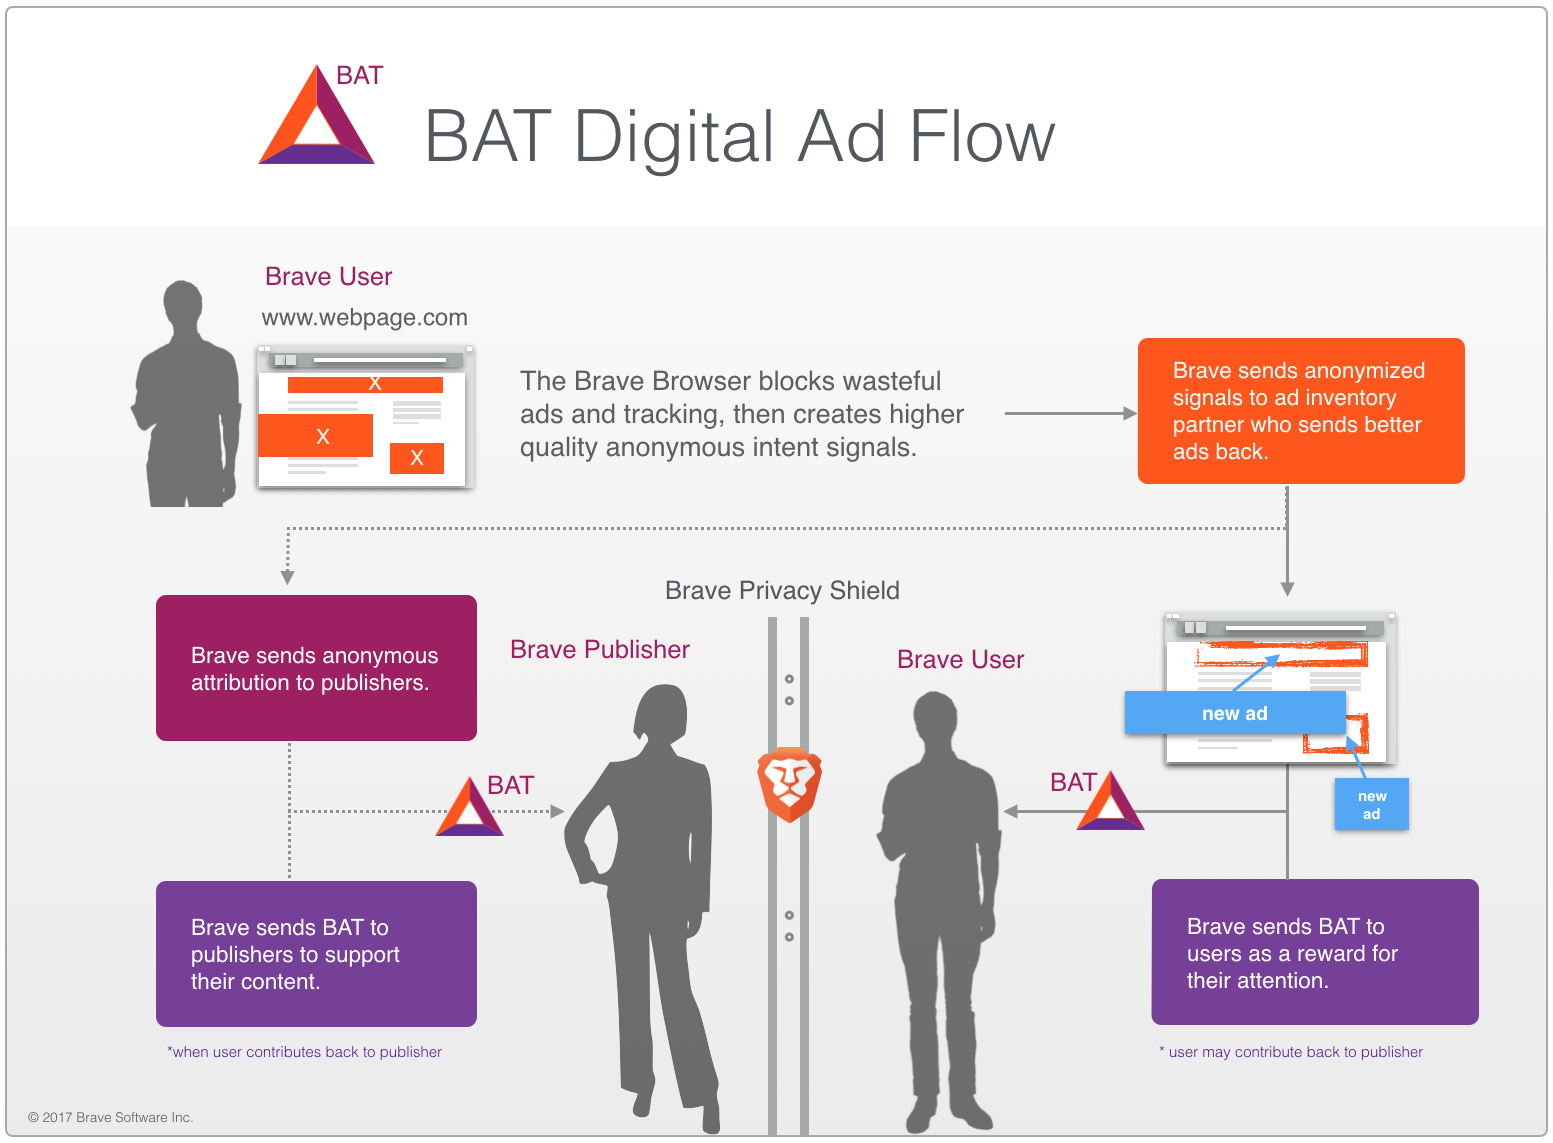
\includegraphics[width=0.9\textwidth]{BAT_digital_ad_flow.png}
\caption{BAT Digital Ad Flow}
\end{center}
\end{figure}



The idea that user attention should have monetary value is familiar to
both publishers and advertisers. The idea of publishers and
particularly users being paid directly for attention bestowed on the
publisher is novel. Since the valuable commodity is user attention, it
makes economic sense that the user be compensated for their
attention. One could justify this as a compensation for the
externalities imposed on users by the advertising ecosystem. One could
also justify this by the fact that one is more likely to perform an
action if one is compensated for it. There is also a guarantee that
the actual user attention is bestowed on the publisher via the
addition of cryptographic contracts built on blockchain to this
advertising stack.  The code is open source and can be reviewed by
researchers and interested parties on the advertiser and publisher sides.

Since the transactions for the first deployment of BAT will happen
through the Brave Ledger, which has privacy and deterministic user
anonymity by design, full transparency can be achieved while user privacy is maintained. While this 
centralized solution should fulfill all economic and technical goals, for further iterations, a fully
decentralized solution could be developed to allow for trustless
auditable transactions.

While paying a user to look at a publisher’s content may seem
heretical to advertisers, the reality is the advertiser is paying
someone. Removing the vast field of middlemen who add no
value to the user/publisher relationship allows for a situation where
the user may be compensated for his valuable attention (made more
valuable and relevant by measures of user interest at the browser)
with no impact to advertiser costs and positive impact to publisher
revenues. From a financial point of view, this could be seen as a
variation on some other kind of short term promotion: advertisers
regularly provide coupons and rebates on products. Promotions do not
solve the problem of informing the user of the advertiser’s product in
the first place. Promotions also don’t induce user loyalty or
engagement. Most CMOs agree that short term sales can be improved with
promotions, but sustainable competitive advantage can’t be achieved
using promotions, hence the use of advertisements. 

\subsection{A Three-Way Coasean Bargain}
\label{sec-8-2}

The three-way Coase theorem is a source of much research interest
among economists. The existence of ``empty cores'' in some situations
have called into question the applicability of the Coase theorem to
real world examples involving multiple distinct players\cite{20}. While there
are many more than three participants in the online ad market, we can
idealize them as consisting of three participants: the advertiser, the
publisher and the user. This analysis is useful for understanding the
game theoretic considerations, for addressing any ``empty core''
arguments against the proposed Coasean bargain, as well as for
illustrating the dire state of the publishing industry. 

We propose the Basic Attention Token (BAT), a cryptographically-secure
token, as the medium of exchange for facilitating this Coasean bargain
while protecting the privacy of the user.

The advertiser wants to purchase user attention. This is broadly
analogous to the ``cost of production'' in the exposition of the Coase
theorem above, whose notation we follow. 

The advertiser values the user attention with price $C^{a}_a$. The publisher wishes to 
monetize the attention $C^{p}_a$ paid to the website. The user who views the website 
values the content of the website with attention $C^{c}_a$.

Advertisers and publishers in the present ecosystem have transaction
costs associated with monetization of attention. Publishers are paid
by advertisers to provide user attention. The intermediaries of the
present system create costs therefore $C^{p}_a <  C^{a}_a$. 

Note, when we talk about ``transaction costs'' apropos the Coase
theorem, we refer to the transaction costs for negotiating a deal
between the players of the Coasean game, therefore, rather awkwardly,
the monetary costs of getting the ad to the publisher is not
considered a ``transaction cost'' per se.

The present advertising ecosystem produces ``social costs'' or attention
pollution as we have discussed above. These social costs are known to
be large. For some large fraction of users (22\% Lumascape state of the
ad industry), the social costs are larger than the attention cost. We
will label the pollution cost following the above example as
$P^{c}_a$. In the present situation, the user will view the
publisher and advertisers’ content so long as $C^{c}_a > P^{c}_a $. 
Every user is different, and of course, the publishers and advertisers
vary as well, but the existence and growth
of a large population of users for whom  $C^{c}_a < P^{c}_a $ indicates that we are
approaching the time where this inequality is always violated. The consequences of this are 
that $ C^{p}_a=0 \iff{(C^{c}_a < P^{c}_a)} $

Since $ C^{c}_a $ is proportional to Publisher profit (and advertiser profit in ``attention''), any value which keeps $C^{c}_a > P^{c}_a $ is advantageous to the Publisher and Advertiser. Effectively the 
advertiser and the publisher combined are the factory
in this argument, and the user owns the pollution rights. However, the
user also values the product of the publisher. In the degenerate case
where $C^{c}_a < P^{c}_a $ the user is also eventually harmed as the
attention economy collapses, and the user takes up other hobbies.


The social cost should be decomposed into its constituent parts. We
have identified the primary components of the social cost in our
exposition of the advertising industry above. Security risk is one
component, $P^{s}$. Hacker networks can place ads in irresponsible ad
exchanges, which could have very large costs for individual users as
well as the publisher who displays those ads. 

Privacy loss is a very important social cost associated with
the advertising landscape as it presently exists, $P^{p}$. Privacy invasions
are presently required by advertisers to make sure the advertisement
is actually viewed by a relevant user. In effect, the advertisers are
paying for something which adds value to the attention. 

Data costs are also a significant part of the social cost of the
present day advertising ecosystem  $P^{d}$. These costs are often borne by the
user as a result of the activities of the middlemen who serve the
advertiser and publisher. These costs seem most trivial, but for many
users, they are among the top causes driving ad blocker adoption. For
all viewers of online ad funded content, considerable time is taken in
dealing with the cost of downloading and executing all the
privacy-violating code. In addition to this cost, for those users who
are using mobile devices, the monetary charges can be significant. It
has been estimated that the top 50 news sites make 16 times less than
the actual charges in data costs of delivering the advertising to the
mobile user of these ads9! Since half or more of the data delivered
by the publisher is advertising-related, half of a data plan can be
hundreds of dollars a year in direct costs to the mobile user. 

Finally, there is the cost to attention produced by the ad itself,
$P^{a}$. In most cases, this is not a large cost, but as it is the thing
actually valued most by advertisers, it should be accounted for
separately. If ads can be made relevant, $P^{a}$ may even be negative. Some
users like looking at certain ads.



\begin{figure}
\begin{center}
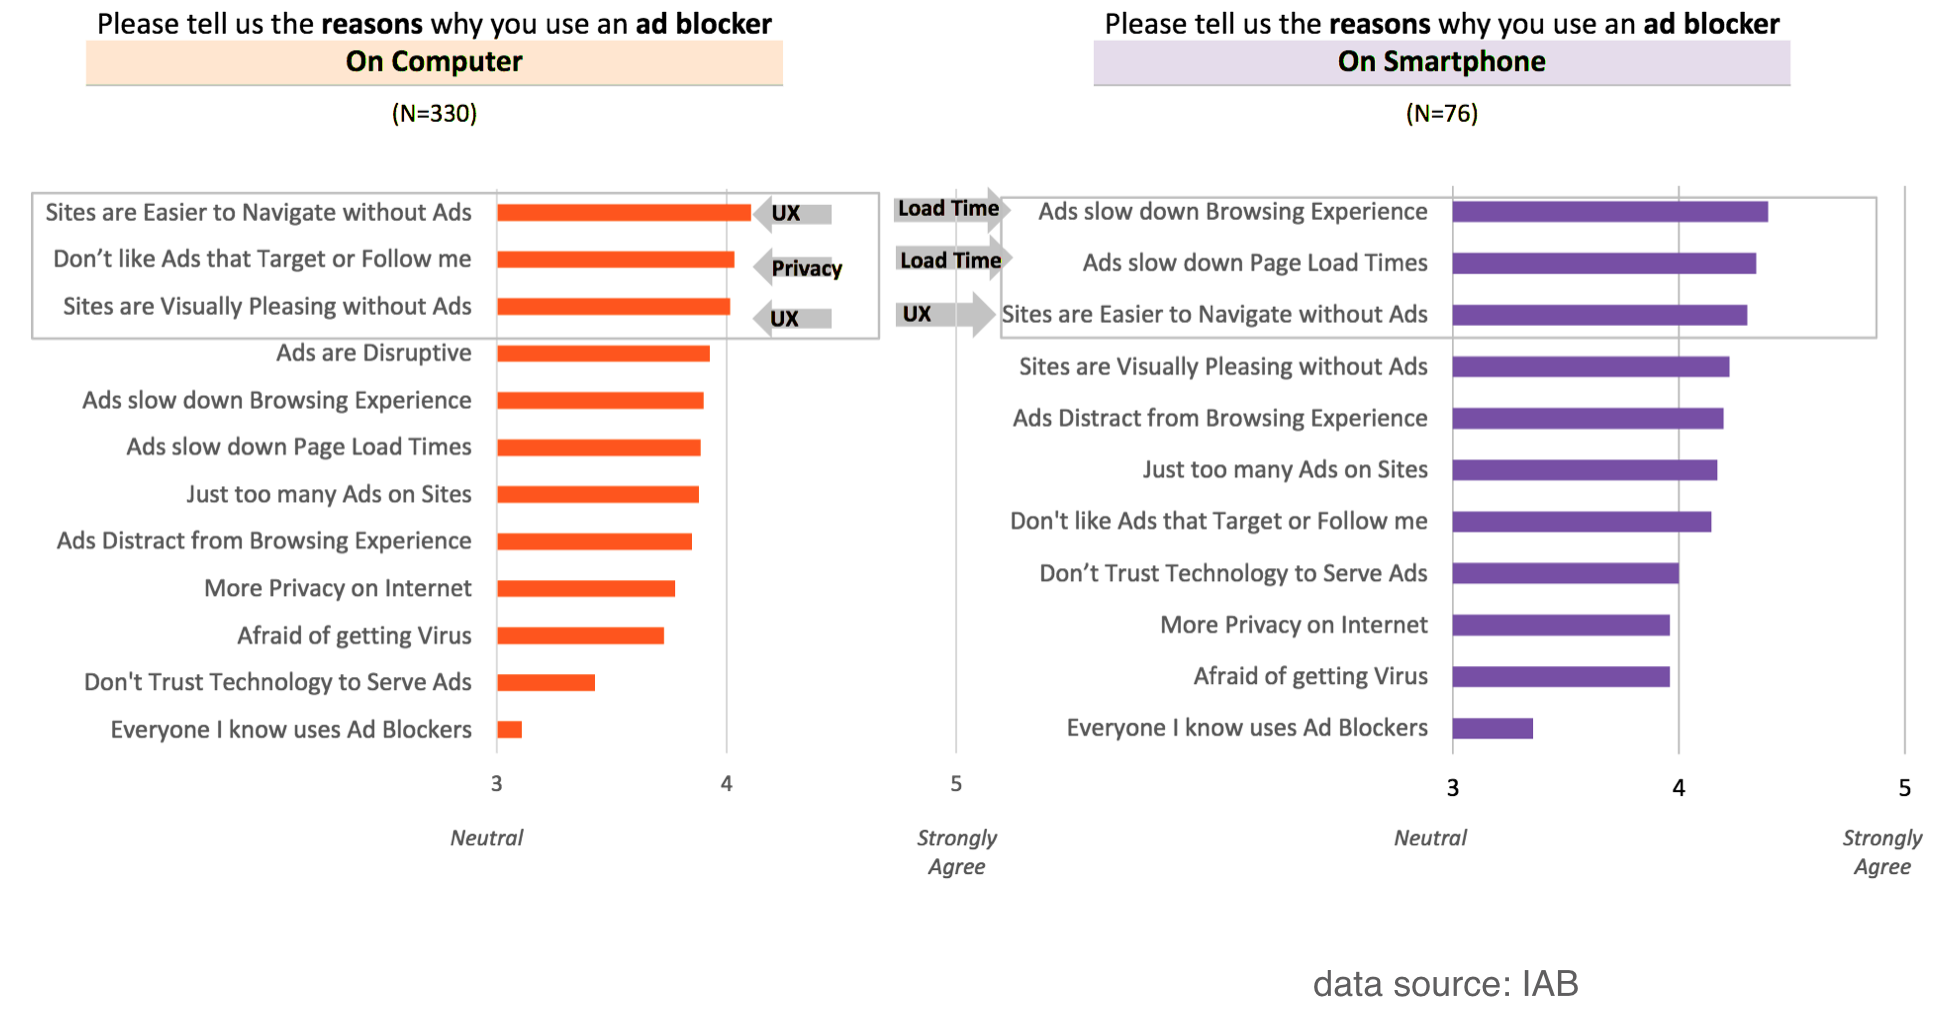
\includegraphics[width=0.9\textwidth]{topreasons_to_block.png}
\caption{Top Reasons to Block Ads: User Experience and Privacy }
\end{center}
\end{figure}





So, our total social cost for the present online ad ecosystem is 
 \[P^{c}_a = P^{a} + P^{d} + P^{p} + P^{s}\]
 For a given value of $P^{a}$ which is the thing actually valued by the
 advertiser, $P^{c}_a $ will always be lower if we can eliminate the other
 factors. A token-based system with anonymizing features would remove $P^{p}$
 entirely. $P^{d}$ will not be entirely mitigated by a token system, as some
 network traffic will take place to service the system and to present
 the ad itself. Since only a few bytes of data will need to be
 transferred to service the token, this cost will effectively only be
 in the downloading of the content of the advertisement; a
 considerable improvement. The use of cryptographic protocols and zero
 knowledge proofs, as well as the use of known publishers and
 advertisers will also lower $P^{s}$ considerably.

So, for a properly privacy protecting token system: 
  \[P^{c}_a(BAT) = P^{a} + P^{d}_{BAT} + P^{s}_{BAT}\]
  To first order approximation,  
  \[P^{c}_a(BAT) = P^{a} + P^{d}_{BAT} \]

The remaining social cost can be eliminated entirely by paying the
user compensation which can be used for other things (for example,
paying a publisher for premium content or apps which relate to the
content). In the simplified game-theoretic case presented here, the
publisher eventually recovers this fraction of the ad spend anyway,
since the publisher is the only place the attention token can be
spent. In a more extensive case where the user can spend the tokens at
other publishers, the revenues taken by the publisher are bounded by
the ratio of the user's take. The way tokens are apportioned in an
advertising event in the proposed scheme, the publisher receives
advertising spend that is much larger than the proposition of
advertising spend they currently receive.

As the user also receives something which is of utility to him, we can
safely declare that $P^{c}_a(BAT)$ is zero or negative, which should encourage users
to view more publisher content. Some may object that the token
acquired by users for their attention activity can only be spent in
the publisher's ``company store,'' but as the token may be saved and
used in different ways, it does have value to the user, just as
airline points and video game tokens do.

The advertiser's spending for a given amount of attention should be
smaller in this ecosystem, since there are fewer social costs
associated with delivering the required attention. In addition, the
advertiser doesn't ever have to pay for social cost to middlemen to
achieve confidence their advertising content was shipped to a relevant
user. Since this situation is better for publishers, and makes for
happier and more ``productive'' users, advertisers should receive more
benefit for their advertising spend.

To summarize, we have used the Coase theorem to demonstrate that the
use of the BAT system offers lower costs to browser users, advertisers
and publishers in the attention economy. Advertisers will receive a
superior share of user attention, along with superior proof of user
engagement. Publishers will receive a larger share of advertising
revenues. Users will receive a superior experience with relevant ads
and a share of advertising revenues.


\subsection{An Analysis of the Stability of the BAT}
\label{sec-8-3}

A model for virtual currency exchange rates was postulated by Dutch
economists von Oordt and Bolt in 2016\cite{22}. The model postulates that the
value of virtual currencies consists of three major factors; the
utility of the virtual currency to make payments, the decision of
forward-looking speculators to regulate the supply of virtual
currency, and the elements that drive user adoption and merchant
acceptance of a virtual currency.   

The argument originates with Fisher's 1911 observation that
speculators may effectively limit the money supply by withdrawing
money from circulation in anticipation of higher future utility. Since
this dynamic particularly applies to limited issuance currencies such
as bitcoin or BAT, it can be an important factor in the pricing for
token sales and stability analysis of virtual currencies.   

For a simple economic system with fixed quantity of currency tokens $M^{BAT}$,
we can write down a transaction quantity relationship: 
\[P^{BAT}_{t} T^{BAT}_{t} = M^{BAT} V^{BAT}_{t} \]

Where $V^{BAT}_{t} $ is velocity of $BAT$, the average number
of times each unit of $BAT$ is used to purchase services within
the defined period of time $t$. $T^{BAT}_{t}$ is the quantity
of services purchased with $BAT$ over the period of time $t$
and $P^{BAT}_{t}$ is the weighted price of the services. 
   
Inserting the exchange rate in terms of $\$$

\[ \frac{P^{BAT}_{t}}{P^{\$}_{t}} T^{BAT}_{t} = M^{BAT} V^{BAT}_{t}\]

Since we can assume the legacy fiat currency is the accounting unit
for all parties involved, we define the exchange rate $S^{\frac{\$}{BAT}}_{t}$, and substitute
in the above equation to give 

 \[S^{\frac{\$}{BAT}}_{t} = \frac{T^{BAT}_{t}}{M^{BAT} V^{BAT}_{t}} \]

If we consider the fraction of currency which is not used in transfer of services, we can postulate a velocity of the fraction of currency which is actually used for settlement $\widehat{V^{BAT}_{t}}$.
Defining $Z^{BAT}_{t}$ to be the number of $BAT$ units not used in transactions.


Since the entire velocity of money in our economy $V^{BAT}_{t}$ is an average
between the currency units used and the units unused for transfer of
services, 
   \[ V^{BAT}_{t} = \frac{M^{BAT}-Z^{BAT}_{t}}{M^{BAT}} \widehat{V^{BAT}_{t}}\]. 

Combining these into the exchange rate

\[ \tag{1} S^{\frac{\$}{BAT}}_{t} = \frac{\widehat{T^{BAT}_{t}}}{(M^{BAT} - Z^{BAT}_{t} ) \widehat{V^{BAT}_{t}}} \]

The exchange rate for BAT tokens is therefore proportional to the
volume of services purchased and inversely proportional to the
currency not used in transactions for the time period $t$. This equation
encapsulates the insight that a lack of money in circulation will
raise the exchange rate.

We now turn our attention to the fraction of BAT which is not used for
exchange. Some of the $Z^{BAT}_{t}$ tokens may
be the result of users forgetting about the small number of tokens
they hold. Some may be due to exchange delays in settlement for legacy
currencies. Overall though, the holders of inactive tokens have
standard ways of evaluating future utility of the tokens in terms of
modern risk management theory.

Since tokens do not bear interest, there is a discounted term
associated with holding a position of size  $z^{BAT}_{t}$ in them.

\[ -R S^{\frac{\$}{BAT}} z^{BAT}_{t} \], where $R$ is the
interest rate discounting in the legacy currency.

If we consider the future expected value of the BAT holdings as the
sum of the future expected value of the position in  BAT
\[ ||S^{\frac{\$}{BAT}}{t+1}|| z^{BAT}_{t}\]

with this discounted interest rate term (where $R$ is the discounting operator),
and the volatility of the future position in BAT scaled by a risk
aversion term $\gamma$, we reach the efficient frontier from modern portfolio
theory.

\[ ||S^{\frac{\$}{BAT}}_{t+1}|| z^{BAT}_{t} -R (S^{\frac{\$}{BAT}}_{t}) z^{BAT}_{t} + \gamma \sigma^{2}(||S^{\frac{\$}{BAT}}_{t+1}||) z^{BAT}_{t} =0\]

Using this standard result, we can solve for the optimal number of
tokens held by an individual during a given time period.

\[ z^{BAT}_{t} =\frac{||S^{\frac{\$}{BAT}}_{t+1}|| -R( S^{\frac{\$}{BAT}}_{t})}{ \gamma \sigma^{2}(||S^{\frac{\$}{BAT}}_{t+1}||) } \]

If we consider all of the people holding BAT at a given time interval $t$
we get the economically efficient number of BAT held for later use.

\[ Z^{BAT}_{t} = N_{t} z^{BAT}_{t} =\frac{||S^{\frac{\$}{BAT}}_{t+1}|| z^{BAT}_{t} -R(S^{\frac{\$}{BAT}}_{t})}{ \frac{\gamma}{N_{t}} \sigma^{2}(||S^{\frac{\$}{BAT}}_{t+1}||) } \]

Since this value can't be negative, we assume that people who hold BAT
have the position that

\[ ||S^{\frac{\$}{BAT}}_{t+1}|| \geq R( S^{\frac{\$}{BAT}}_{t})\]

hence, using our above relationship, we get the relationship between the expected future value of the BAT, the interest rate and the velocity of transfers in the BAT economy:

\[R^{-1} (||S^{\frac{\$}{BAT}}_{t+1}||) \geq \frac{T^{BAT}_{t}}{M^{BAT} V^{BAT}_{t}} \]

So, people hold BAT if the discounted expected value exceeds the
hypothetical value of the current exchange rate. So, the exchange rate
as a function of future expected value of BAT is

\[\tag{2} S^{\frac{\$}{BAT}}_{t} = R^{-1} (||S^{\frac{\$}{BAT}}_{t+1}|| -\frac{\gamma}{N_t}Z^{BAT}_{t} \sigma^{2}(||S^{\frac{\$}{BAT}}_{t+1} ||) )\]
    
Thus, the BAT holdings are the discounted expected future exchange
rate minus the risk premium for the uncertainty in future value of the
BAT.

If the model holds, {1} and {2} can be used to define supply and
demand for BAT. Since $M^{BAT}$ is not time dependent in the case of BAT, the
time varying exchange rate can be readily understood in terms of BAT
transactions and opinions on future utility of BAT transactions. As
BAT transactions increase, the exchange rate becomes dominated by the
transactions rather than future expectations of utility. This dynamic
has been observed in maturing virtual currencies as well as various
other in-house token systems.

While models are imprecise, this model argues for long term price
stability in a token mediated economy. 

\printbibliography


\end{document}
